\documentclass[review]{elsarticle}
\usepackage{lineno,hyperref}
\usepackage{amsmath}
\usepackage{amssymb}
\usepackage{latexsym}
\usepackage{amsfonts}
\usepackage{mathrsfs}
\usepackage{natbib}
\usepackage{graphicx} % figuras
\usepackage[export]{adjustbox} % loads also graphicx
\usepackage{float}
\usepackage[font=footnotesize]{caption}
\usepackage{wrapfig}
\biboptions{numbers,sort&compress}
\modulolinenumbers[5]

\journal{Journal of \LaTeX\ Templates}

%%%%%%%%%%%%%%%%%%%%%%%
%% Elsevier bibliography styles
%%%%%%%%%%%%%%%%%%%%%%%
%% To change the style, put a % in front of the second line of the current style and
%% remove the % from the second line of the style you would like to use.
%%%%%%%%%%%%%%%%%%%%%%%

%% Numbered
%\bibliographystyle{model1-num-names}

%% Numbered without titles
%\bibliographystyle{model1a-num-names}

%% Harvard
%\bibliographystyle{model2-names.bst}\biboptions{authoryear}

%% Vancouver numbered
%\usepackage{numcompress}\bibliographystyle{model3-num-names}

%% Vancouver name/year
%\usepackage{numcompress}\bibliographystyle{model4-names}\biboptions{authoryear}

%% APA style
%\bibliographystyle{model5-names}\biboptions{authoryear}

%% AMA style
%\usepackage{numcompress}\bibliographystyle{model6-num-names}

%% `Elsevier LaTeX' style
\bibliographystyle{elsarticle-num}
%%%%%%%%%%%%%%%%%%%%%%%

\begin{document}

\begin{frontmatter}

\title{On POD-based Deflation Vectors for DPCG applied to porous media problems}
%\tnotetext[mytitlenote]{Fully documented templates are available in the elsarticle package on \href{http://www.ctan.org/tex-archive/macros/latex/contrib/elsarticle}{CTAN}.}

%% Group authors per affiliation:
%\author{, ,\fnref{myfootnote}}
%\address{Mekelweg 4, Delft}
%\fntext[myfootnote]{TU Delft}

%% or include affiliations in footnotes:
\author[mymainaddress]{G. B. Diaz Cortes\corref{mycorrespondingauthor}}
\cortext[mycorrespondingauthor]{Corresponding author}
\ead{g.b.diazcortes@tudelft.nl}
\author[mymainaddress]{C. Vuik}
%\ead[url]{www.elsevier.com}
\author[mysecondaryaddress] {J.D. Jansen}
%\ead[url]{www.elsevier.com}


\address[mymainaddress]{Faculty of Electrical Engineering, Mathematics and Computer Science, Delft University of Technology,
Mekelweg 4, 2628 CD Delft, The Netherlands
}
\address[mysecondaryaddress]{Faculty of Civil Engineering and Geosciences, Delft University of Technology,
Stevinweg 1, 2628 CN Delft, The Netherlands}

\begin{abstract}
     We study fast and robust iterative solvers for large systems of  linear equations resulting from
     simulation of flow trough strongly heterogeneous porous media. We propose the use of preconditioning and deflation techniques, based on 
     information obtained from the system, to reduce the time spent in the solution of the linear system.\\
     An important question when using deflation techniques is how to find good deflation vectors, which lead to a decrease in the number of iterations 
     and a small increase in the required computing time per iteration. In this paper, we propose the use of deflation vectors
     based on a POD-reduced set of snapshots. We investigate convergence and the properties of the resulting methods. 
     Finally, we illustrate these theoretical results with numerical experiments.  
 We consider compressible and incompressible single-phase flow in a layered model with  variations in the 
 permeability layers up to $10^{3}$ and the SPE 10 benchmark model with a contrast in permeability coefficients of $10^{7}$. Using deflation for the incompressible problem, we reduce the number of iterations to 1 or 2 iterations. With deflation, for the compressible problem, we get a reduction up to $\sim 80\%$ in the number of iterations when compared with only-preconditioned solver.
\end{abstract}

\begin{keyword}
\texttt{elsarticle.cls}\sep \LaTeX\sep Elsevier \sep template
\MSC[2010] 00-01\sep  99-00
\end{keyword}

\end{frontmatter}

\linenumbers

\section{Introduction}
Often, most computational time in the simulation of multi-phase flow through porous media is taken 
  up by the solution of the pressure equation. 
This involves, primarily, solving large systems of linear equations as 
part of the iterative solution of the time and space discretized governing nonlinear partial differential 
equations. The time spent in solving the linear systems depends on the size of the problem and the heterogeneity, i.e. the spatial
variations of rock permeability values within the medium (Permeability is an inverse measure of the  resistance to flow which is related to the porosity and the pore structure of the rock). Solution of problems with extreme contrasts in the
permeability values may lead to very large computing times. \\
Iterative methods are known to be the best option to solve such extreme problems. However, sometimes iterative methods are not sufficient to solve these problems in a reasonable amount of time. As the systems become larger or ill-conditioned, finding a way to accelerate the convergence of these methods becomes necessary. Preconditioning is a way to accelerate convergence, but new preconditioning techniques still need to be developed to improve the performance of iterative methods \cite{Vuik02,Benzi02}.
Reduced Order Models (ROM) have also been studied to improve computational efficiency by reducing the model size without losing essential information \cite{Antoulas05,Schilders08,Quarteroni14}. 
A potential ROM to reduce the computing time for large-scale problems is Proper Orthogonal 
Decomposition (POD), a method that has been investigated for flow problems in porous media in \cite{Heijn04,Vermeulen04,Mark06,Doren06,Cardoso09,Astrid11,Krogstad11,Efendiev12,Jiang13,Pasetto16} among others. 
The use of a POD-based preconditioner for acceleration of the solution is proposed by Astrid et al.
\cite{Astrid11} to solve the pressure equation resulting from two-phase reservoir simulation, by Jiang et al. \cite{Jiang13} for a similar application and by Pasetto 
et al. \cite{Pasetto16} for groundwater flow models. \\
The POD method requires the computation of a series of 'snapshots' which are solutions of the problem with slightly 
different parameters or well inputs. Astrid et al. \cite{Astrid11} use snapshots in the form of solutions of the pressure equation computed in a small number of short pre-simulations, prior to the actual simulation,\ with diverse well configurations, reporting promising speed ups with factors between three and five. They note that the overhead required to pre-compute the POD solutions implies that the method will be particularly attractive when many solutions of near-similar simulation models are required. A similar approach is followed by Jiang \cite{Jiang13}, who concludes that POD-based pressure preconditioning does not appear to be an ideal choice because of its dependence on the differences between the right-hand sides (forcing terms) used in the pre-simulations and the actual simulation. The snapshots computed by Pasetto et al. \cite{Pasetto16} are solutions of the previous time steps in the full-model.
Once the snapshots are computed, the POD method is used to obtain a set of basis 
vectors that capture the most relevant features of the system, which can be used to speed-up the subsequent simulations.\\
The method of Pasetto at al. \cite{Pasetto16} is partly based on the work of Markovinovic and Jansen \cite{Mark06} who use a similar, but more restricted, approach in which the acceleration is 
achieved by only improving the initial guess.\\
Problems with high contrast between the permeability coefficients are sometimes approached through the 
use of deflation techniques, see, e.g., \cite{Vuik99}. These techniques involve the search 
of good deflation vectors, which are usually problem-dependent. In \cite{Vuik99}, subdomain based deflation 
vectors are used for layered problems with a large contrast between permeability coefficients. However, 
these deflation vectors cannot be used if the distribution of the permeability coefficients  is not 
structured, as is usually the case in reservoir simulation models; see, e.g., the well-known SPE 10 benchmark problem \cite{Christie01}.\\
Algebraic Multigrid (AMG)\cite{Klie07}, Multi-level and Domain Decomposition \cite{Tang09} preconditioners have been studied in combination deflation techniques to accelerate the convergence of iterative methods.
In \cite{Mark06,Astrid11} and \cite{Pasetto16}, after computing a basis from the 
previously obtained snapshots, the solution is computed in the subspace generated by this basis and then projected 
back to the original high-dimensional system. Carlberg et al. \cite{Carlberg15} also use POD to obtain information 
from the system, in particular, the previous time step solutions. Then, a Krylov-subspace is constructed using the 
information obtained previously.\\
Following the ideas of \cite{Astrid11,Mark06,Pasetto16,Carlberg15}, we propose the use of POD of many snapshots 
to capture the system's behavior and combine this technique with deflation to accelerate the convergence of 
an iterative Krylov method.
In this work, instead of computing the solution in a low dimensional subspace, the basis obtained with POD is 
proposed as an alternative choice for the deflation vectors 
to accelerate the convergence of the pressure solution in reservoir simulation.  \\
This work is divided into six sections. 
  Section \ref{fpm} is devoted to a detailed description of the models used to simulate flow through a porous medium. In Section \ref{syseq}, we present some theory about the linear solvers used in this work and we introduce preconditioning 
  and deflation techniques. 
  In Section \ref{POD} we present some theory about POD. We prove two lemmas that will help us in the choice of good deflation vectors for the 
  incompressible case in Section \ref{as}.\\
 In Section \ref{numexp} we present numerical experiments. We describe the problem that is studied, the solver and the preconditioning and deflation techniques used to speed up the solver. The results are also presented
 in this section.
 Finally, we end with the conclusions.
 \section{Flow through porous media}\label{fpm}
Petroleum reservoirs are layers of sedimentary rock, which vary in terms of their grain size and mineral clay contents. The volume fraction of the rock in-between the grains, i.e. the void space, is called $rock$
$porosity$, a scalar quantity indicated with $\phi$.\\
The ability of the rock to transmit a single fluid when the void space is completely filled with fluid
is known as $rock$ $permeability$, a tensor quantity indicated with ${K}$. \\
Reservoir simulation is a way to analyze and predict the fluid behavior in a reservoir. The description of subsurface flow simulation involves two types of models: geological (static) and flow (dynamic) models. The static model is used to describe spatial properties of the reservoir, i.e., the porosities and permeabilities which are parameters for the dynamic model. 
The dynamic model is subsequently used to predict fluid pressures and flow taking into account mass conservation and Darcy's law, an empirical, simplified version of the momentum conservation equations. The corresponding equations used to describe single-phase flow through a porous medium are (see, e.g., \cite{Aziz79,Chen06,Jansen13})  :
\begin{equation}\label{eq:ce}
\frac{\partial (\rho \phi)}{\partial t}+ \nabla \cdot ( \rho {v})=q, \qquad v=-\frac{K}{\mu}(\nabla p-\rho g\nabla z),
\end{equation}
or
\begin{equation}\label{eq:ce1}
\frac{\partial (\rho \phi)}{\partial t}- \nabla \cdot \left( \frac{\rho{K}}{\mu}(\nabla {p}-\rho g\nabla z)\right)=q,
\end{equation}
where the pressure $p$ is the primary unknown, $g$ is the constant of gravity, $d$ is the reservoir depth,
$\rho$ and $\mu$ are the fluid density and viscosity and $q$ is a source term (i.e., an injection or production well). The fluid density $\rho=\rho(p)$ and the rock porosity $\phi=\phi(p)$ can be pressure-dependent.
Rock porosity is related to the pressure via the rock compressibility. The relation is given by:
\begin{equation*}
 c_r=\frac{1}{\phi}\frac{d\phi}{dp}=\frac{d(ln(\phi))}{dp},
\end{equation*}
If the rock compressibility is constant, the previous equation can be integrated as:
\begin{equation}\label{eq:por}
 \phi(p)=\phi_0 e^{c_r(p-p_0)}.
\end{equation}
The fluid density and the pressure are related via the fluid compressibility $c_f$, according to:
\begin{equation*}\label{eq:fc}
 c_f=\frac{1}{\rho}\frac{d\rho}{dp}=\frac{d(ln(\rho))}{dp}.
\end{equation*}
If the fluid compressibility is constant, the previous equation can be integrated as:
\begin{equation}\label{eq:rhoeq}
 \rho(p)=\rho_0 e^{c_f({p}-{p}_0)}.
\end{equation}
To solve Equation \eqref{eq:ce1}, it is necessary to supply conditions at the boundary of the domain. While for parabolic equations, we also need to impose initial conditions. Boundary and initial conditions will be discussed later for each problem.   \\
\textbf{Incompressible fluid}\\
If the density and the porosity are not pressure-dependent in Equation \eqref{eq:ce1}, we have an incompressible model, where density and porosity do not change over time. Therefore, the incompressible model is time-independent. Assuming no gravity terms and a fluid with constant viscosity, Equation \eqref{eq:ce1} then becomes:
\begin{equation}\label{eq:cel}
-\frac{\mathbf{\rho}}{\mu}\nabla \cdot \left({K} \nabla p\right)=q.
\end{equation}
\emph{Discretization}\\
The spatial derivatives are approximated using a finite difference scheme with cell central 
differences. For a 3D model, taking a mesh with a uniform grid size $\Delta x$, $\Delta y$, $\Delta z$ where $(i,j,l)$ is the center 
of the cell
in the position $i$ in the $x$ direction, $j$ in the $y$ direction, and $l$ in the $z$ direction
($x_i,y_j,z_l$) and where $p_{i,j,l}=p(x_i,y_j,z_l)$ is 
the pressure at this point.
\\ For the $x$ direction, we have (see, e.g., \cite{Aziz79,Chen06,Jansen13}):
\begin{align*}
&\frac{\partial}{\partial x}\left(k\frac{\partial p}{\partial x}\right) = 
\frac{\Delta}{\Delta x}\left(k\frac{\Delta p}{\Delta x}\right) +\mathscr{O}(\Delta x^2)\\
&=\frac{ k_{i+\frac{1}{2},j,l}(p_{i+1,j,l}-p_{i,j,l})-k_{i-\frac{1}{2},j,l}(p_{i,j,l}-p_{i-1,j,l})}{\left( \Delta x\right)^2}+\mathscr{O}(\Delta x^2),
\end{align*}
where $k_{i-\frac{1}{2},j,l}$ is the harmonic average of the permeability for cells 
$(i-1,j,l)$ and $(i,j,l)$:
\begin{equation}\label{eq:ha}
 k_{i-\frac{1}{2},j,l}=\frac{2}{\frac{1}{ k_{i-1,j,l}}+\frac{1}{ k_{i,j,l}}}.
\end{equation}
After discretization, Equation \eqref{eq:cel}, together with boundary conditions, can be written as:
 \begin{equation}\label{eq:cel1}
\mathbf{T}\mathbf{p} = \mathbf{q},
\end{equation}
where $\mathbf{T}$ is known as the transmissibility matrix with elements in adjacent grid cells. The $transmissibility$ ($T_{i-\frac{1}{2},j,l}$) between grid cells $(i-1,j,l)$ and $(i,j,l)$ is defined as \cite{Cordazzo02}:
\begin{equation}\label{eq:htrans}
 T_{i-\frac{1}{2},j,l}=\frac{2\Delta y \Delta z}{\mu\Delta x}k_{i-\frac{1}{2},j,l},
\end{equation} 
System \eqref{eq:cel1} is a linear system that can be solved with iterative or direct methods. For the solution of this system, it is necessary to define boundary conditions in all boundaries of the domain. These conditions can be prescribed pressures 
(Dirichlet conditions), flow rates (Neumann conditions) or a combination of these (Robin conditions).  \\\\
\textbf{Compressible fluid}\\
If the fluid is compressible with a constant compressibility, the density depends on the pressure Equation \eqref{eq:rhoeq}. Therefore, Equations \eqref{eq:ce} become:
\begin{equation}\label{eq:ce2}
\frac{\partial (\rho(p) \phi)}{\partial t}+ \nabla \cdot ( \rho(p) {v})=q, \qquad v=-\frac{K}{\mu}(\nabla p-\rho(p) g\nabla z),
\end{equation}
\emph{Discretization}\\
Using backward Euler time discretization, Equations \eqref{eq:ce2} are approximated by:
\begin{equation*}
 \frac{(\mathbf{\phi}\mathbf{\rho}(p))^{n+1}-(\mathbf{\phi}\mathbf{\rho}(p))^{n}}{\Delta t^n}
 +\nabla \cdot (\mathbf{\rho}({p}) v)^{n+1}={q}^{n+1},
\end{equation*}
\begin{equation}\label{eq:ce3}
{v}^{n+1}= -\frac{{K}}{\mu^{n+1}}(\nabla({p}^{n+1})-g\mathbf{\rho}^{n+1}\nabla{z}).
\end{equation}
Assuming no gravity terms, constant fluid viscosity and constant rock porosity, Equations \eqref{eq:ce3}
become:
\begin{equation}\label{eq:ce4}
 \mathbf{\phi}\frac{\mathbf{\rho}({p}^{n+1})
 -\mathbf{\rho}({p}^{n})}{\Delta t^n}
 -\frac{1}{\mu}\nabla \cdot (\mathbf{\rho}({p}^{n+1}) 
 {K}\nabla{p}^{n+1})+{q}^{n+1}=0.
\end{equation}
Due to the dependence of $\rho$ on the pressure, the latter is a nonlinear equation for $p$ that can be linearized with, e.g., the Newton-Raphson (NR) method.
Equation \eqref{eq:ce4} can be discretized in space, using a finite differences scheme. After spatial discretization, Equation \eqref{eq:ce4} reads:
\begin{equation}\label{eq:ce5}
\mathbf{V}\mathbf{{p}}^{n,n+1}+\mathbf{T}\mathbf{p}^{n+1}=\mathbf{q}^{n+1}.
\end{equation}
We note that in a more general case, where also the porosity is pressure-dependent, a slightly more complex, mass conservative formulation is usually employed; see refs.\cite{Aziz79,Chen06,Jansen13}. As in the incompressible case, we need to define boundary condition to solve Equation \eqref{eq:ce5}. Dirichlet, Neumann or Robin boundary conditions can be used. For this problem, we also have a derivative with respect to time. Therefore, it is also necessary to specify the initial conditions that are the pressure values of the reservoir at the beginning of the simulation.\\\\
\textbf{Well model}\\
In reservoirs, wells are typically drilled to extract or inject fluids. Fluids are injected into a well or produced from a well at constant rate or constant bottom-hole pressure (bhp).\\
 When the bhp is prescribed, the flow rates into or from the wells are usually compute with the aid of a well model. 
 A widely used model is Peaceman's model, that takes into account the bhp and the average grid pressure in the block containing the well. 
This model is a linear relationship between the bhp and the flow rate in a well. For a cell $(i,j,l)$ that contains a well, this relationship is given by:
\begin{equation}\label{eq:wellm}
{q}_{(i,j,l)}={I}_{(i,j,l)}({p}_{(i,j,l)}-{p}_{bh(i,j,l)}),
\end{equation}
where ${I}_{(i,j,l)}$ is the productivity or injectivity index of the well, ${p}_{(i,j,l)}$ is the reservoir pressure in the cell 
where the well is located, 
and ${p}_{bh(i,j,l)}$ is a prescribed pressure inside the well. \\
\emph{Incompressible fluid}\\
Using the well model for an incompressible fluid, Equation \eqref{eq:cel1} transforms into:
 \begin{equation}\label{eq:celw1}
\mathbf{T}\mathbf{p} = \mathbf{I}_w(\mathbf{p}-\mathbf{p}_{bh}),
\end{equation}
where $\mathbf{I}_w$ is a diagonal matrix containing the productivity or injectivity indices of the wells present in the reservoir. 
The diagonal elements are zero for cells without wells and have the value of the well index for each cell containing a well.\\
\emph{Compressible fluid}\\
For a compressible fluid, using the well model, Equation \eqref{eq:ce5} reads:
\begin{equation}\label{eq:cew4}
 {\phi}\frac{{\rho}(\mathbf{p}^{n+1})
 -{\rho}(\mathbf{p}^{n})}{\Delta t^n}
 -\frac{1}{\mu}\nabla \cdot ({\rho}(\mathbf{p}^{n+1}) 
 \mathbf{K}\nabla\mathbf{p}^{n+1})+\mathbf{I}_w^{n+1}(\mathbf{p}^{n+1}-\mathbf{p}_{bhp}^{n+1})=\mathbf{0}.
\end{equation}\\
\textbf{Solution procedure for compressible flow}\\
As mentioned before, for the compressible problem, we have a nonlinear system that depends on the pressure at the time step $n$ and the pressure at time step $n+1$:
\begin{equation}\label{eq:NR}
 \mathbf{g}(\mathbf{p}^{n+1};\mathbf{p}^n)=0.
\end{equation}
This nonlinear system can be solved with the NR method, the system for the $(k+1)$-th NR iteration is:
$$\mathbf{J}(\mathbf{p}^k)\delta\mathbf{p}^{k+1}=-\mathbf{g}(\mathbf{p}^k;\mathbf{p}^n),
\qquad \mathbf{p}^{k+1}=\mathbf{p}^k+\delta \mathbf{p}^{k+1},$$
where $\mathbf{J}(\mathbf{p}^k)=\frac{\partial \mathbf{g}(\mathbf{p}^k;\mathbf{p}^n)}{\partial \mathbf{p}^k}$ is the 
Jacobian matrix, and $\delta \mathbf{p}^{k+1}$ is the NR update at iteration step $k+1$.\\
Therefore, the linear system to solve is:\\
\begin{equation}\label{eq:lsJ}
\mathbf{J}(\mathbf{p}^k)\delta \mathbf{p}^{k+1}=\mathbf{b}(\mathbf{p}^k).
\end{equation}
with $\mathbf{b}(\mathbf{p}^k)$ being the function evaluated at iteration step $k$, $\mathbf{b}(\mathbf{p}^k)=-\mathbf{g}(\mathbf{p}^k;\mathbf{p}^n)$.\\
The procedure to solve a compressible flow problem consists of three stages. During the first stage, we increase the time with one time step and solve Equation \eqref{eq:cew4} for the new time. Because of the nonlinearity of Equation \eqref{eq:cew4} we use an iterative Newton Raphson procedure that involves linearization at each iteration, i.e., we perform a series of iterations to find the 
zeros of Equation \eqref{eq:NR}. For every NR iteration the linear system in Equation \eqref{eq:lsJ} is solved. 
In this work, the solution of the linear system is performed with iterative methods (see Section \ref{syseq}). A summary of 
this procedure is presented in Algorithm 1.

\begin{table}[!h]\centering
\begin{minipage}{1\textwidth}
\begin{tabular}{ |l| } 
\hline
\textbf{Algorithm 1}\\
\hline
\hline
\hspace{0.5cm}\textbf{for} $t=0,...,$    \hspace{52mm}    \%Time integration \\
\hspace{1cm} Select time step\\
\hspace{1cm}\textbf{for} $NR\_iter=0,...,$    \hspace{34mm}    \%NR iteration\\
 \hspace{1.5cm} Find zeros of $\mathbf{g}(\mathbf{p}^{n+1};\mathbf{p}^n)=0$\\
\hspace{1.5cm}\textbf{for} $lin\_iter=0,...,$    \hspace{31mm}    \%Linear iteration \\
\hspace{2cm}Solve $\mathbf{J}(\mathbf{p}^k)\delta \mathbf{p}^{k+1}=\mathbf{b}(\mathbf{p}^k)$ for each NR iteration\\
\hspace{1.5cm}\textbf{end}\\
\hspace{1cm}\textbf{end}\\
\hspace{0.5cm}\textbf{end}\\
\hline
\end{tabular}
\end{minipage}
\end{table}

\section{Iterative solution methods}\label{syseq}
When simulating single-phase flow through a porous medium, we obtain a linear system
\begin{equation}\label{eq:linsys}
 \mathbf{A}\mathbf{x}=\mathbf{b},
\end{equation}
for both compressible and incompressible models. 
Since $\mathbf{A}$ is SPD, we choose Conjugate Gradient (CG) as iterative method accelerated with the Incomplete Cholesky preconditioner. In this work, we also study the acceleration with deflation techniques. In this section, we give a brief overview of the methods. \\\\
\textbf{Conjugate Gradient Method}\\
Given a starting solution $\mathbf{x}^0$ and the residual defined by $\mathbf{r}^k=\mathbf{b}-\mathbf{A}\mathbf{x}^k$, we define the Krylov subspace 
$\mathcal{K}_k(\mathbf{A},\mathbf{r}^0)=span\{\mathbf{r}^0,\mathbf{A}\mathbf{r}^0,\dots,\mathbf{A}^{k-1}\mathbf{r}^0\}$ and $\mathbf{x}^k\in \mathbf{x}^0+\mathcal{K}_k(\mathbf{A},\mathbf{r}^0)$ has a minimal error measured in the $\mathbf{A}$-norm for all approximations contained in $\mathbf{x}^0+\mathcal{K}_k(\mathbf{A},\mathbf{r}^0).$ The error of this approximation is bounded by:
\begin{equation}\label{eq:conv1}
 ||\mathbf{x}-\mathbf{x}^{k+1}||_\mathbf{A}\leq 2||\mathbf{x}-\mathbf{x}^{0}||_\mathbf{A} 
 \left( \frac{\sqrt{\kappa_2(\mathbf{A})}-1}{\sqrt{\kappa_2(\mathbf{A})}+1} \right)^{k+1}
 \footnote{The condition number $\kappa_2(\mathbf{A})$ is defined as  $\kappa_2(\mathbf{A})=
 \frac{\sqrt{\lambda_{max}(\mathbf{A}^T\mathbf{A})}}{\sqrt{\lambda_{min}(\mathbf{A}^T\mathbf{A})}}$. 
 If $\mathbf{A}$ is SPD, $\kappa_2(\mathbf{A})=\frac{\lambda_{max}(\mathbf{A})}{\lambda_{min}(\mathbf{A})}$.}.
 \end{equation}
 The pseudo code for CG is given in Algorithm 2.\\
 \begin{table}[!h]
\begin{tabular}{ |l| } 
\hline
  \textbf{Algorithm 2} Conjugate Gradient (CG) method, solving $\mathbf{A}\mathbf{x}=\mathbf{b}$.\\
  \hline
 \hline
\\
Give an initial guess $\mathbf{x}^0$. \\Compute $\mathbf{r}^0=\mathbf{b}-\mathbf{A}\mathbf{x}^0$ and set $\mathbf{p}^0=\mathbf{r}^0$.\\

\hspace{0.5cm}\textbf{for} $k=0,...,$ until convergence\\
 \hspace{1cm} $\alpha^k=\frac{(\mathbf{r}^{k},\mathbf{r}^{k})}{(\mathbf{A}\mathbf{p}^k,\mathbf{p}^k)}$\\
\hspace{1cm} $\mathbf{x}^{k+1}=\mathbf{x}^k+\alpha^k\mathbf{p}^k$\\
\hspace{1cm}$\mathbf{r}^{k+1}=\mathbf{r}^k-\alpha^k\mathbf{A}\mathbf{p}^k$\\
\hspace{1cm}$ \beta^k=\frac{(\mathbf{r}^{k+1},\mathbf{r}^{k+1})}{(\mathbf{r}^k,\mathbf{r}^k)}$\\
\hspace{1cm}$\mathbf{p}^{k+1}=\mathbf{r}^{k+1}+\beta^k\mathbf{p}^k$\\
\hspace{0.5cm}\textbf{end}\\
\hline
\end{tabular}
\end{table}

\textbf{Preconditioning}\\
To accelerate the convergence of a Krylov method, one can transform the system into
another one containing an iteration matrix with a better spectrum , i.e, a smaller condition number. 
This can be done by multiplying the system \eqref{eq:linsys} by a matrix $\mathbf{M}^{-1}.$
\begin{equation}\label{eq:precon}
 \mathbf{M}^{-1}\mathbf{A}\mathbf{x}=\mathbf{M}^{-1}\mathbf{b}.
\end{equation}
The new system has the same solution but can provide a substantial reduction of the condition number. 
For this preconditioned system, the error is bounded by:
\begin{equation}\label{eq:convp}
 ||\mathbf{x}-\mathbf{x}^{k}||_\mathbf{A}\leq 2||\mathbf{x}-\mathbf{x}^{0}||_\mathbf{A} 
 \left( \frac{\sqrt{\mathbf{\kappa}(\mathbf{M}^{-1}\mathbf{A})}-1}{\sqrt{\mathbf{\kappa}(\mathbf{M}^{-1}\mathbf{A})}+1} \right)^{k}.
\end{equation}
$\mathbf{M}$ is chosen as an $SPD$ matrix such that $\mathbf{\kappa}(\mathbf{M}^{-1}\mathbf{A})\leq \mathbf{\kappa}(\mathbf{A}),$ and $\mathbf{M}^{-1}\mathbf{b}$ is cheap to compute.\\\\
\textbf{Deflation}\\
Deflation is used to annihilate the effect of extreme eigenvalues on the convergence of an iterative method (\cite{Vuik99}). 
Given an $SPD$ matrix $\mathbf{A} \in \mathbb{R}^{n \times n}$, for a given matrix $\mathbf{Z}\in \mathbb{R}^{n\times m}$ the deflation matrix $\mathbf{P}$ is defined as follows (\cite{Tang08,Tang09}):
$$\mathbf{P}=\mathbf{I}-\mathbf{A}\mathbf{Q}, \qquad \mathbf{P} \in \mathbb{R}^{n \times n}, \qquad \mathbf{Q} \in \mathbb{R}^{n \times n},$$
where
$$\mathbf{Q}=\mathbf{Z}\mathbf{E}^{-1}\mathbf{Z}^T, \qquad \mathbf{Z} \in \mathbb{R}^{n \times m}, \qquad \mathbf{E} \in \mathbb{R}^{m \times m}, $$
with
$$\mathbf{E}=\mathbf{Z}^T\mathbf{A}\mathbf{Z}.$$
The matrix $\mathbf{E}$ is known as the $Galerkin$ or $coarse$ matrix that has to be invertible. 
If $\mathbf{A}$ is $SPD$ and $\mathbf{Z}$ is full rank then $\mathbf{E}$ is invertible. 
The full rank matrix $\mathbf{Z}$ is called the $deflation-subspace$ matrix, 
and it's columns are the
$deflation$ vectors or $projection$ vectors.\\
\textbf{Deflated PCG Method}\\
\hspace{0.5cm}To obtain the solution of linear system \eqref{eq:linsys}, we have to solve the deflated system (see Appendix \ref{a4}):
\begin{align}\label{eq:defsol}
\mathbf{P}\mathbf{A} \hat{\mathbf{x}}=\mathbf{P}\mathbf{b},
\end{align}
with the CG method, for the deflated solution $\hat{\mathbf{x}}$. 
This deflated the solution is related to the solution $\mathbf{x}$ of the original system as (see Appendix \ref{a4}):
\begin{equation}\label{eq:xfromxh}
    \mathbf{x}=\mathbf{Q}\mathbf{b}+\mathbf{P}^T\mathbf{\hat{x}}.
\end{equation}
The deflated linear system can also be preconditioned by an $SPD$ matrix $\mathbf{M}$. After preconditioning, the deflated preconditioned system to solve with CG is \cite{Tang09}:
$$\tilde{\mathbf{P}} \tilde{\mathbf{A}} \hat{\tilde{\mathbf{x}}}=\tilde{\mathbf{P}}\tilde{\mathbf{b}},$$
where:
\begin{equation*}
 \tilde{\mathbf{A}}=\mathbf{M}^{-\frac{1}{2}}\mathbf{A}\mathbf{M}^{-\frac{1}{2}}, \qquad \hat{\tilde{\mathbf{x}}}=\mathbf{M}^{\frac{1}{2}}\hat{\mathbf{x}}, \qquad
 \tilde{\mathbf{b}}=\mathbf{M}^{-\frac{1}{2}}\mathbf{b}
\end{equation*}
This method is called the Deflated Preconditioned Conjugate Gradient $DPCG$ method.
In practice $\mathbf{M}^{-1}\mathbf{P}\mathbf{A}\mathbf{x}=\mathbf{M}^{-1}\mathbf{P}\mathbf{b}$ is computed and the error is bounded by:
\begin{equation*}
 ||\mathbf{x}-\mathbf{x}^{i+1}||_\mathbf{A}\leq 2||\mathbf{x}-\mathbf{x}^{0}||_\mathbf{A} \left( \frac{\sqrt{\mathbf{\kappa}_{eff}(\mathbf{M}^{-1}\mathbf{P}\mathbf{A})}-1}{\sqrt{\mathbf{\kappa}_{eff}(\mathbf{M}^{-1}\mathbf{P}\mathbf{A})}+1} \right)^{i+1},
\end{equation*}
were $\mathbf{\kappa}_{eff}=\frac{\lambda_{max}(M^{-1}PA)}{\lambda_{min}(M^{-1}PA)}$ is the effective condition 
number and $\lambda_{min}(M^{-1}PA)$ is the smallest non-zero eigenvalue of $M^{-1}PA$.

\subsection{Choices of Deflation Vectors}
The deflation method is used to remove the effect of the most unfavorable eigenvalues
of $\mathbf{A}$. If the matrix $\mathbf{Z}$ contains eigenvectors corresponding to the unfavorable 
eigenvalues, the convergence of the 
iterative method is achieved faster. However, to obtain and to apply the eigenvectors is costly in view of memory and CPU time.
Therefore, a good choice of the matrix $\mathbf{Z}$ that efficiently approximates the eigenvectors is essential
for the applicability of the method.\\
A good choice of the deflation vectors is usually problem-dependent. Available information on the system is, in general,
used to obtain these vectors.
Most of the techniques used to choose deflation vectors are based on approximating eigenvectors, 
recycling \cite{Clemens04}, subdomain deflation vectors \cite{Vuik02} or multigrid and 
multilevel based deflation techniques \cite{Tang09,Smith96}. A summary of these techniques is given below.
\begin{description}
 \item [Recycling Deflation.] A set of search vectors previously used is reused to build the deflation-subspace 
 matrix \cite{Clemens04}. 
The vectors could be, for example, $q-1$
solution vectors of the linear system with different right-hand sides or of different time steps.
The matrix $\mathbf{Z}$ containing these solutions is:
$$\mathbf{Z}=[\mathbf{x}^{(1)},\mathbf{x}^{(2)},...,\mathbf{x}^{(q-1)}].$$
 \item [Subdomain Deflation.] The domain is divided into several subdomains,
 using domain decomposition techniques or taking into account the properties of the problem.
For each subdomain, there is a deflation vector that contains ones for cells in the 
subdomain and zeros for cells outside \cite{Vuik02}.
 \item [Multi Grid and Multilevel Deflation.] For the multigrid and multilevel methods, 
 the prolongation and restriction matrices are used to pass from one level or grid to another. 
These matrices can be used as the deflation-subspace matrices $\mathbf{Z}$ \cite{Tang09}.
\end{description}
\newpage
\section{Proper Orthogonal Decomposition (POD)}\label{POD}
As mentioned before, in this work we want to combine deflation techniques and Proper Orthogonal Decomposition (POD) to reduce the number of iterations necessary to solve the linear system obtained from reservoir simulation in a cheap and automatic way. In this section, we give a brief overview of the POD method.\\
The POD method is a Model Order Reduction (MOR) method, where a high-order model is projected onto a space
spanned by a small set of orthonormal basis vectors.
The high dimensional variable $\mathbf{x} \in \mathbb{R}^n$
is approximated by a linear combination of $l$ orthonormal basis vectors \cite{Astrid11}:
\begin{equation}\label{eq4}
  \mathbf{x}\approx \sum_{i=1}^lc_i \mathbf{\psi}_i,
\end{equation}
where $\psi_i \in \mathbb{R}^n$ are the basis vectors and $c_i$ are their corresponding coefficients.
In matrix notation, equation \eqref{eq4} is rewritten as :
$$\mathbf{x}\approx \Psi\mathbf{c},$$
where $\Psi=[\psi_1 \text{ }\psi_2 \text{ }.. \text{ }\psi_l]$, $\Psi \in \mathbb{R}^{n\times l}$ 
is the matrix containing the basis vectors, and $\mathbf{c} \in \mathbb{R}^l$ is the vector 
containing the coefficients of the basis vectors. \\
The basis vectors $\psi_i$ are computed from a set of 'snapshots' $\{ \mathbf{x_i}\} _{i=1,..,m}$, 
obtained by simulation or experiments \cite{Mark06}. 
In POD, the basis vectors $\{ \mathbf{\psi} _j \} ^l _{j=1},$ are $l$ eigenvectors corresponding to 
the largest eigenvalues $\{ \mathbf{\sigma} _j \} ^l _{j=1}$ of the data snapshot correlation matrix $\mathbf{R}$.
\begin{equation}\label{eq:POD}
\mathbf{R}:= \frac{1}{m}\mathbf{X}\mathbf{X}^T \equiv \frac{1}{m} \sum_{i=1}^m \mathbf{x}_i \mathbf{x}_i^T,
\qquad \mathbf{X}:=[\mathbf{x}_1,\mathbf{x}_2,...\mathbf{x}_m],
\end{equation}
where $\mathbf{X}\in \mathbb{R}^{n\times m}$ is an SPSD matrix containing the previously obtained snapshots.
The $l$ eigenvectors should contain almost all the variability of the snapshots. 
Usually, they are chosen as the eigenvectors of the maximal number ($l$) of eigenvalues satisfying \cite{Mark06}:
\begin{equation}
\frac{\sum_{j=1}^l\sigma_j}{\sum_{j=1}^m\sigma_j}\leq \alpha, \qquad 0<\alpha \leq 1,
\end{equation}
with $\alpha$ close to 1. The eigenvalues $\sigma_j$ are ordered from large to small with $\sigma_1$
the largest eigenvalue of $\mathbf{R}$. 
It is not necessary to compute the eigenvalues from $\mathbf{X}\mathbf{X}^T$, but instead, it is possible to compute the eigenvalues of the much smaller matrix $\mathbf{X}^T\mathbf{X}$ (see Appendix \ref{a3}). \\
% The covariance matrix $\bar{\mathbf{R}}$ (see Equation \eqref{eq:POD1}) is frequently used instead of $\mathbf{R}$.
% \begin{equation}\label{eq:POD1}
% \bar{\mathbf{R}}:=  \frac{1}{m} \sum_{i=1}^m (\mathbf{x}_i -\bar{\mathbf{x}})(\mathbf{x}_i-\bar{\mathbf{x}})^T,
% \qquad \bar{\mathbf{x}}:=\frac{1}{m} \sum_{i=1}^m\mathbf{x}_i.
% \end{equation}
In this study, we normalize the snapshots, so $||\mathbf{x}_i||_2=1.$
\section{Deflation vector analysis.}\label{as}
As mentioned in Section \ref{syseq}, it is important to choose 'good' deflation vectors if we want to speed up an iterative method.\\ 
We can use solutions of systems slightly different from the original (snapshots) as deflation vectors.
For this, we need to choose a way of selecting these snapshots. The idea behind this selection is to obtain a small number of snapshots and, at the same time,
obtain the largest amount of information from the system.\\
In this section, two lemmas are proved. The lemmas are helpful to select the systems used to obtain the snapshots.\\\\
\textbf{Lemma 1.} 
Let $\mathbf{A} \in \mathbb{R}^{n\times n}$ be a non-singular matrix, and $\mathbf{x}$ be the solution of:
\begin{equation}\label{eq:ls}
\mathbf{A}\mathbf{x}=\mathbf{b}.
\end{equation}
Let $ \mathbf{x}_i, \mathbf{b}_i \in \mathbb{R}^{n},$ $i=1,...,m,$ be
vectors linearly independent ($l.i.$) and 
\begin{equation}\label{eq:lieq}
\mathbf{A}\mathbf{x}_i=\mathbf{b}_i.
\end{equation}
The following equivalence holds
\begin{equation}\label{eq:equiv}
\mathbf{x}=\sum_{i=1}^m {c}_i\mathbf{x}_i \qquad
\Leftrightarrow \qquad
\mathbf{b}=\sum_{i=1}^m {c}_i\mathbf{b}_i.
\end{equation}
Proof $\Rightarrow$
\begin{equation}\label{eq:equiv1}
\mathbf{x}=\sum_{i=1}^m {c}_i\mathbf{x}_i 
\Rightarrow 
\mathbf{b}=\sum_{i=1}^m {c}_i\mathbf{b}_i.
\end{equation}
Substituting $\mathbf{x}$ from \eqref{eq:equiv1} into $\mathbf{A}\mathbf{x}=\mathbf{b}$ leads to:
\begin{align*}
\mathbf{A}\mathbf{x}&=\sum_{i=1}^m \mathbf{A}{c}_i\mathbf{x}_i=\mathbf{A}(c_1\mathbf{x}_1+...+c_m\mathbf{x}_m).
\end{align*}
Using the linearity of $\mathbf{A}$ the equation above can be rewritten as:
\begin{align}\label{eq:bc}
\mathbf{A}c_1\mathbf{x}_1+...+\mathbf{A}c_m\mathbf{x}_m
=c_1\mathbf{b}_1+...+c_m\mathbf{b}_m=\mathbf{B}\mathbf{c}.
\end{align}
where $\mathbf{B} \in \mathbb{R}^{n\times m},$ $\mathbf{c} \in \mathbb{R}^{m}$, and the columns of $\mathbf{B}$
are the vectors $\mathbf{b}_i$.\\
From \eqref{eq:ls} and \eqref{eq:bc} we get:
\begin{align*}
\mathbf{A}\mathbf{x}=\mathbf{b}=c_1\mathbf{b}_1+...+c_m\mathbf{b}_m=\sum_{i=1}^m {c}_i\mathbf{b}_i.\\
\end{align*}
Proof $\Leftarrow $
\begin{equation}\label{eq:equiv2}
\mathbf{x}=\sum_{i=1}^m {c}_i\mathbf{x}_i\Leftarrow \mathbf{b}=\sum_{i=1}^m {c}_i\mathbf{b}_i .
\end{equation}
Substituting $\mathbf{b}$ from \eqref{eq:equiv2} into $\mathbf{A}\mathbf{x}=\mathbf{b}$ leads to:
\begin{align}%\label{eq:equiv21}
\mathbf{A}\mathbf{x}&=\sum_{i=1}^m {c}_i\mathbf{b}_i.
\end{align}
Since $\mathbf{A}$ is non-singular, multiplying \eqref{eq:lieq} and \eqref{eq:equiv2} by $\mathbf{A}^{-1}$ we obtain:
\begin{align*}%\label{eq:equiv21}
\mathbf{x}_i&=\mathbf{A}^{-1}\mathbf{b}_i,
\end{align*}
\begin{align*}%\label{eq:equiv21}
\mathbf{x}&=\mathbf{A}^{-1}\sum_{i=1}^m {c}_i\mathbf{b}_i=\sum_{i=1}^m {c}_i\mathbf{A}^{-1}\mathbf{b}_i,
\end{align*}
then 
\begin{align}\label{eq:equiv21}
\mathbf{x}=\sum_{i=1}^m {c}_i\mathbf{x}_i.
\end{align}
\begin{flushright}
$\boxtimes $                
\end{flushright}
\textbf{Lemma 2.}
If the the deflation matrix $\mathbf{Z}$ is constructed with a set of $m$ vectors 
\begin{equation}
 \mathbf{Z}=
\begin{bmatrix}
\mathbf{x}_1&...&...&\mathbf{x}_m
\end{bmatrix}, 
\end{equation}
such that $\mathbf{x}=\sum_{i=1}^m {c}_i\mathbf{x}_i$, with $\mathbf{x}_i$ $l.i.$, then the solution of
system \eqref{eq:ls} is obtained with one iteration of DCG.\\
Proof.\\
The relation between $\mathbf{\hat{x}}$ and $\mathbf{x}$ is given in Equation \eqref{eq:xfromxh}:
\begin{equation*}
    \mathbf{x}=\mathbf{Q}\mathbf{b}+\mathbf{P}^T\mathbf{\hat{x}}. 
\end{equation*}
For the first term $\mathbf{Q}\mathbf{b}$, taking $\mathbf{b}=\sum_{i=1}^m {c}_i\mathbf{b}_i$ we have:

\begin{align*}
\mathbf{Q}\mathbf{b}&=\mathbf{Z}\mathbf{E}^{-1}\mathbf{Z}^T\left(\sum_{i=1}^m {c}_i\mathbf{b}_i\right)\\
&=\mathbf{Z}(\mathbf{Z}^T\mathbf{A}\mathbf{Z})^{-1}\mathbf{Z}^T\left(\sum_{i=1}^m {c}_i\mathbf{A}\mathbf{x}_i\right)\qquad \text{using Lemma 1}\\
&=\mathbf{Z}(\mathbf{Z}^T\mathbf{A}\mathbf{Z})^{-1}\mathbf{Z}^T\left( \mathbf{A}\mathbf{x}_1{c}_1+...+\mathbf{A}\mathbf{x}_m{c}_m\right) \\
&=\mathbf{Z}(\mathbf{Z}^T\mathbf{A}\mathbf{Z})^{-1}\mathbf{Z}^T(\mathbf{A}\mathbf{Z}\mathbf{c})  \\
&=\mathbf{Z}(\mathbf{Z}^T\mathbf{A}\mathbf{Z})^{-1}(\mathbf{Z}^T\mathbf{A}\mathbf{Z})\mathbf{c} \\
&=\mathbf{Z}\mathbf{c}= c_1\mathbf{x}_1+c_2\mathbf{x}_2+c_3\mathbf{x}_3+c_4\mathbf{x}_4+c_5\mathbf{x}_5\\
& =\sum_{i=1}^m {c}_i\mathbf{x}_i=\mathbf{x}.
\end{align*}
Therefore,
\begin{equation}\label{eq:xqb}
\mathbf{x}=\mathbf{Q}\mathbf{b},
\end{equation}
is the solution to the original system.\\ 
For the second term of Equation \eqref{eq:xfromxh}, $\mathbf{P}^T\mathbf{\hat{x}}$, we compute $\mathbf{\hat{x}}$ from Equation \eqref{eq:defsol}:
\begin{align*}
    \mathbf{P}\mathbf{A}\hat{\mathbf{x}}&=\mathbf{P}\mathbf{b}\\
    \mathbf{A}\mathbf{P}^T\hat{\mathbf{x}}&=(\mathbf{I}-\mathbf{A}\mathbf{Q})\mathbf{b} \qquad \text{using \ref{defprop} f) and definition of $\mathbf{P}$,}\\
        \mathbf{A}\mathbf{P}^T\hat{\mathbf{x}}&=\mathbf{b}-\mathbf{A}\mathbf{Q}\mathbf{b}\\
        \mathbf{A}\mathbf{P}^T\hat{\mathbf{x}}&=\mathbf{b}-\mathbf{A}\mathbf{x}=0 \qquad \text{taking $\mathbf{Q}\mathbf{b}=\mathbf{x}$ from above,}\\
          \mathbf{P}^T\hat{\mathbf{x}}&=0 \qquad \text{as $\mathbf{A}$ is invertible.}
\end{align*}
Then we have obtain the solution 
$$\mathbf{x}=\mathbf{Q}\mathbf{b}+\mathbf{P}^T\mathbf{\hat{x}}=\mathbf{Q}\mathbf{b},$$ 
in one step of DCG.
\begin{flushright}
$\boxtimes $                
\end{flushright}
\subsection{Accuracy of the snapshots.}\label{accs}
If we use an iterative method to obtain an approximate solution $\mathbf{x}^k$ for the system $\mathbf{A}\mathbf{x}=\mathbf{b},$ we cannot compute the relative error $e_r$
(Equation \eqref{eq:re}) of the approximation with respect to the true solution because the true solution is unknown, 
\begin{equation}\label{eq:re}
 e_r=\frac{||\mathbf{x}-\mathbf{x}^k||_2}{||\mathbf{x}||_2}.
\end{equation}
Instead, we compute the relative residual $r_r$ (Equation \eqref{eq:rr}), 
\begin{equation}\label{eq:rr}
r_r= \frac{||\mathbf{r}^k||_2}{||\mathbf{b}||_2}\leq \epsilon,
\end{equation}
and we set a stopping criterium $\epsilon$ or tolerance, that is related to the relative error as follows \cite{Saad03} (see Appendix \ref{a2}),
$$\frac{||\mathbf{x}-\mathbf{x}^k||_2}{||\mathbf{x}||_2}\leq \kappa_2(\mathbf{A}) \epsilon=r_r.$$
Various tolerance values can be used in the experiments for the snapshots as well as for the solution of the original system. \\
If the maximum relative residual for the snapshots ($\mathbf{x}_i$) is $\epsilon=10^{-\eta}$, then, the error in the snapshots is given by
$$\frac{||\mathbf{x}_i-\mathbf{x}_i^k||_2}{||\mathbf{x}_i||_2}\leq \kappa_2(\mathbf{A})\times 10^{-\eta}=r_r.$$

From Equation \eqref{eq:equiv21}, if we compute $m$ snapshots with an iterative method such that the solution of $\mathbf{x}$ is a linear combination of these vectors, after one iteration of DCG we obtain
$$\mathbf{x}^{1}=\sum_{i=1}^m {c}_i\mathbf{x}_i^{1(i)},$$
where $\mathbf{x}_i^{1(i)}$ is the approximated solution of the snapshot $i$ after one DCG iteration.\\ 
The error of this solution is given by:
$$\frac{||\mathbf{x}-\mathbf{x}^1||_2}{||\mathbf{x}||_2}=
\frac{||\sum_{i=1}^m {c}_i(\mathbf{x}_i-\mathbf{x}_i^{1})||_2}{||\sum_{i=1}^m {c}_i\mathbf{x}_i||_2}\leq
\frac{\sum_{i=1}^m| {c}_i|\times \kappa_2(\mathbf{A})\times 10^{-\eta}}{||\sum_{i=1}^m {c}_i\mathbf{x}_i||_2},
$$
which means that the approximation has an error of the order $\kappa_2(\mathbf{A})\times10^{-\eta}.$
\\From Lemma 2 we know that if we use the snapshots $\mathbf{x}_i$ as deflation vectors, for the deflation method the solution is given by (Equation \eqref{eq:xqb}): $$\mathbf{x}=\mathbf{Q}\mathbf{b}.$$ 
If the approximation $\mathbf{x}^1$ has an error of the order $\kappa_2(\mathbf{A})\times10^{-\eta}$, then, the solution achieved with the deflation method will have the same error, 
$$\mathbf{Q}\mathbf{b}-\mathbf{x}^1=\kappa_2(\mathbf{A})\times10^{-\eta}.$$
Therefore, it is important to take into account the condition number of the matrix to estimate the accuracy of the deflation vectors.
\subsection{Boundary conditions.}
From Lemma 2, we know that if we use as deflation vectors a set of $m$ snapshots $$\mathbf{Z}=[\mathbf{x}_1\qquad ...\qquad \mathbf{x}_m],$$ such that $\mathbf{x}=\sum_{i=1}^m {c}_i\mathbf{x}_i$, where $\mathbf{x}$ is the solution of the system $\mathbf{A}\mathbf{x}=\mathbf{b}$, the solution of the latter system is achieved with one DCG iteration. \\
In our application, only a small number ($m$) of elements of the right-hand side vector $\mathbf{b}$
can be changed. This implies that every $\mathbf{b}$ can be written as $\mathbf{b}=\sum_{i=1}^m {c}_i\mathbf{b}_i.$ Using Lemma 1, this implies that $\mathbf{x}$ is such that 
$\mathbf{x}\in span\{ \mathbf{x}_1, ...,  \mathbf{x}_m\}$, which is called the solution span.
Therefore, it is necessary to find the solution span of the system, such that the sum of the elements in the solution span and the sum of right-hand sides give as result the original system. In this section, we explore the subsystems that should be chosen, depending on the boundary conditions of the original system. 
\subsubsection*{{Neumann Boundary conditions}}
When we have Neumann boundary conditions everywhere, the resulting matrix $\mathbf{A}$ is singular, and
$\mathbf{A}[1\quad 1\quad ...\quad 1\quad 1]^T=\mathbf{0},$ $Ker(\mathbf{A})=span([1\quad 1\quad ...\quad 1\quad 1]^T)$. 
Note that $\mathbf{A}\mathbf{x}=\mathbf{b}$ has only a solution if $\mathbf{b}\in span\{\mathbf{a}_1,...,\mathbf{a}_n\}$ (with $\mathbf{a}_i$ the $i-th$ column of $\mathbf{A}$), which is equivalent to $\mathbf{b}\perp Ker(\mathbf{A}) $ \cite{Strang09}.
This implies that if we have $m$ sources with value ${s}_i$ for the vector $\mathbf{b}_i$, we need that 
$$\sum_{j=1}^ m {s}^{j}_i=0.$$
Then, for each nonzero  right-hand side we need to have at least two sources. Therefore, we can have at most $m-1$ linearly independent right-hand sides $\mathbf{b}_{i}$ containing two sources.\\
This means that the solution space has dimension $m-1$ and it can be spanned by $ span\{\mathbf{x}_1,...,\mathbf{x}_{m-1}\}$.
Each of these subsystems will have the same no-flux conditions (Neumann) in all the boundaries.
As the original system is a linear combination of the subsystems (Lemma 1), the deflation vectors can be chosen as the solutions corresponding to the subsystems. Therefore, the deflation matrix will be given by:
$$\mathbf{Z}=[\mathbf{x}_1\qquad ...\qquad \mathbf{x}_{m-1}],$$
and if the accuracy of the snapshots used as deflation vectors is high enough (see Section \ref{accs}), the solution is expected to be achieved in one DCG iteration. 
\subsubsection*{{Dirichlet Boundary conditions}}
In this case, the right-hand side of the system can contain the values of the boundary $\mathbf{b}_b$ and the sources of the system $\mathbf{s}_i$. 
If we have $m$ sources, as in the previous case, the right-hand side will be given by:
$$\mathbf{b}=\sum_{i=1}^{m} {c}_i\mathbf{s}_i+\mathbf{b}_b.$$
The subsystems will be $m+1$, where one of them corresponds to the boundary conditions
 $\mathbf{A}\mathbf{x}_b=\mathbf{b}_b,$
 and the other $m$ will correspond to the sources
$\mathbf{A}\mathbf{x}_i=\mathbf{s}_i.$
Therefore, snapshot $m+1$ will be the solution $\mathbf{x}_b$ of the system with no sources and the Dirichlet boundary conditions of the original system. The other $m$ snapshots will correspond to the $m$ sources with homogeneous Dirichlet boundary conditions. Then, the solution space will be given by $ span\{\mathbf{x}_1,...,\mathbf{x}_{m},\mathbf{x}_b\}$.
If we use the solution of the $m+1$ snapshots as deflation vectors, with the correct accuracy, we will obtain the solution within one DCG iteration.

\section{Numerical experiments}\label{numexp}
\subsection{Model.}\label{modpro}
\hspace{0.5cm} We study the solution of systems of linear equations resulting from the discretization of elliptic and parabolic partial differential equations for the description of single-phase flow through a porous medium. 
The solution of the linear system is performed with the Conjugate Gradient method preconditioned with Incomplete Cholesky (ICCG) and the Deflated Conjugate Gradient method preconditioned with Incomplete Cholesky (DICCG).
We propose the use of snapshots and snapshots-based POD basis vectors as deflation vectors for the above-mentioned method.\\
In the present section, we give a general overview of the experiments we perform, but the specifications
 are presented below for each problem separately. We solve the elliptic problem (incompressible flow) and the parabolic problem (compressible flow). Neumann boundary conditions (no-flux) are imposed for an academic layered problem and for the SPE 10 benchmark problem.
\\ \\
\emph{The model}\\
The experiments simulate flow through a porous medium with a constant porosity field of 0.2.
We model incompressible and compressible single-phase flow.
For the single-phase model the following properties of the fluid are used:
\begin{itemize}
 \item $\mu = 1$ $cp$,
 \item $\rho = 1014$ $kg/m^3$,
\end{itemize}
In the compressible case, the compressibility of the fluid is:
\begin{itemize}
 \item $c= 1 \times 10^{-3}$.
\end{itemize}
The matrices corresponding to the linear systems $\mathbf{A}$ and right-hand sides $\mathbf{b}$ are obtained with the Matlab Reservoir Simulation Toolbox (MRST) \cite{Lie13}.
\\ \\
\emph{Snapshots}\\
As mentioned before, for the DICCG method we need a set of deflation vectors. In the first series of
experiments (incompressible model), the deflation vectors are 
solutions of the system with various wells configurations. These solutions, 
called $snapshots$, are obtained with the ICCG method. 
For the compressible problem, the snapshots are the solutions of the previous time steps with the same well configuration. 
We also propose the use of a POD basis as deflation vectors, obtained from the previously computed snapshots for the incompressible and compressible cases.
As tolerance or stopping criterium, we use the relative residual, defined as the 2-norm of the residual of the $k^{th}$ iteration divided by 
the 2-norm of the right-hand side of the preconditioned or deflated system: 
$$r_r=\frac{||\mathbf{M}^{-1}r^k||_2}{||\mathbf{M}^{-1}b||_2}\leq \epsilon.$$
\subsection{Incompressible Problem}

We simulate single-phase flow through a porous medium, for an incompressible fluid (see Equation \eqref{eq:cel1}), with the previously mentioned characteristics. Homogeneous Neumann boundary conditions are imposed on all boundaries. This model contains five wells, four on the corners and one in the center of the domain. \\
A set of four linearly independent snapshots is used as deflation vectors (DICCG$_4$). We also use a linearly dependent set of 15 snapshots (DICCG$_5$) and a 4-vectors POD basis obtained from these 15 snapshots (DICCG$_{POD_4}$). We set the same boundary conditions as in the original problem for all the snapshots.
The four linearly independent snapshots ($\mathbf{z}_1$-$\mathbf{z}_4$) are obtained giving a value of zero to one well and non-zero values to the other wells, such that the sum of the well pressures equals zero. The set of 15 snapshots are all possible combinations of wells such that the flow-in equals the flow-out of the reservoir. The snapshots and the solutions are obtained with a tolerance of $10^{-11}$. \\
A summary of the well configurations is presented in Table \ref{table:sc}.
\renewcommand{\arraystretch}{1}
\begin{table}[!ht]\centering
\begin{minipage}{.45\textwidth}
\vspace{-10pt}
\centering
\begin{tabular}{ |c|c|c|c|c|c|} 
 \hline
  \multicolumn{6}{|c|}{System configuration} \\ 
  \hline
  \multicolumn{6}{|c|}{Well pressures (bars)}\\
  \hline
  &$W1$ &$W2$ &$W3$ &$W4$ &$W5$ \\
  \hline
&-1 & -1& -1& -1& 4\\
\hline
\multicolumn{6}{|c|}{Snapshots } \\
\multicolumn{6}{|c|}{ (linearly independent)} \\
\hline
 &$W1$ &$W2$ &$W3$ &$W4$ &$W5$ \\
  \hline

$\mathbf{z}_1$& 0&-1 &-1 &-1 &3 \\
$\mathbf{z}_2$& -1&0 &-1 &-1 &3  \\
$\mathbf{z}_3$& -1&-1 &0 &-1 &3  \\
$\mathbf{z}_4$& -1&-1 &-1 &0 &3  \\
 \hline
 \end{tabular}
\label{table:case2}\end{minipage}%
\hspace{15pt}
 \begin{minipage}{.45\textwidth}
 \begin{tabular}{ |c|c|c|c|c|c|} 
 \hline
 \multicolumn{6}{|c|}{Additional snapshots} \\
 \multicolumn{6}{|c|}{ (linearly dependent)} \\
\hline
 &W1 &W2 &W3 &W4 &W5 \\
  \hline
$\mathbf{z}_5$& -1&-1 &-1 &-1 &4  \\
$\mathbf{z}_6$& -1&0 &0 &-1 &2  \\
$\mathbf{z}_7$& -1&-1 &0 &0 &2  \\
$\mathbf{z}_8$& -1&0 &-1 &0 &2  \\
$\mathbf{z}_9$& 0&-1 &-1 &0 &2  \\
$\mathbf{z}_{10}$& 0&-1 &0 &-1 &2  \\
$\mathbf{z}_{11}$& 0&0 &-1 &-1 &2  \\
$\mathbf{z}_{12}$& -1&0 &0 &0 &1  \\
$\mathbf{z}_{13}$& 0&-1 &0 &0 &1  \\
$\mathbf{z}_{14}$& 0&0 &-1 &0 &1  \\
$\mathbf{z}_{15}$& 0&0 &0 &-1 &1  \\
 \hline
 \end{tabular}

\end{minipage}\caption{Table with the well configurations of the system and the snapshots.}
\vspace{-10pt}\label{table:sc}
\end{table}

\normalsize
\newpage
\emph{\textbf{Heterogeneous permeability layers}}\\

\begin{wrapfigure}{R}{4.5cm}
\centering 
\vspace{-10pt}
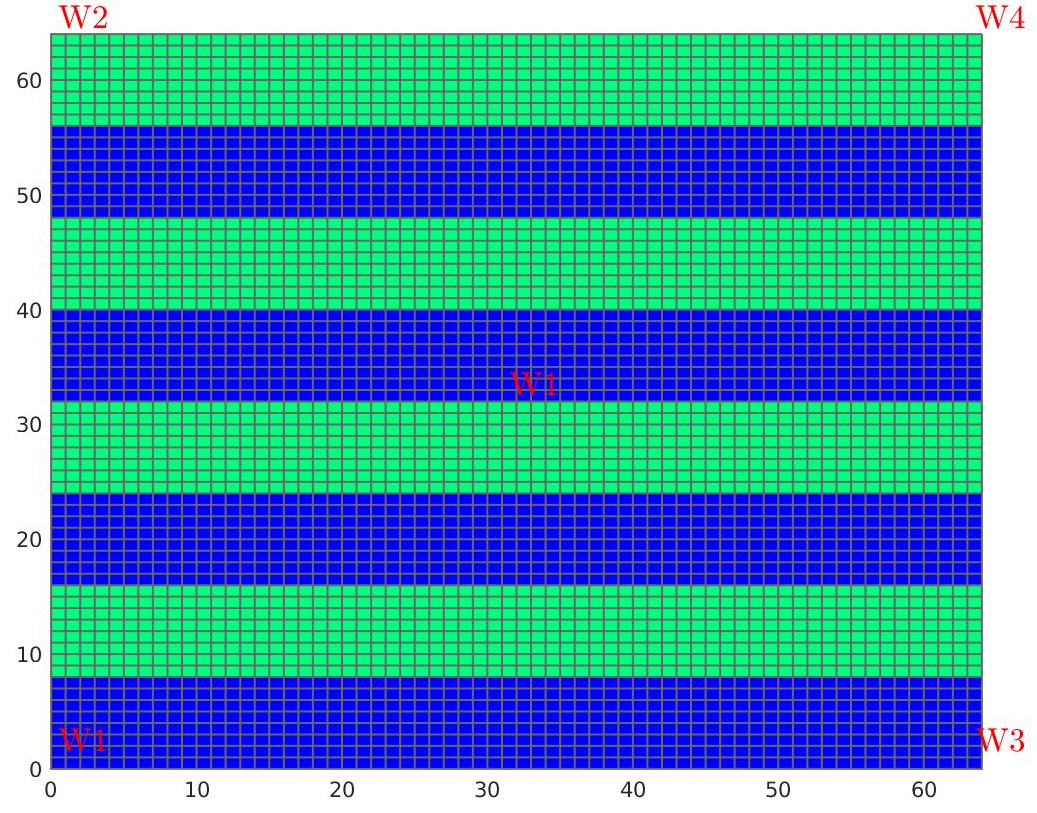
\includegraphics[width=4cm,height=4cm,keepaspectratio]{images/perm64.jpg}
 %\vspace{-25pt}
\caption{ Heterogeneous permeability, 5 wells.}\label{fig:hep_2}
\vspace{-10pt}
\end{wrapfigure} 
A Cartesian grid of $64\times64$ grid cells and length ($L_x$,$L_y$) of $70\times70$ $m^2$ with 8 layers of the same size is studied. Four layers have a permeability  $\sigma_1$ and they are followed by a layer with a different permeability value $\sigma_2$ (see Figure \ref{fig:hep_2}). The permeability of one set of layers is set to $\sigma_1=1mD$, the permeability of the other set $\sigma_2$ is varied. 
Therefore, the contrast in permeability between the layers $(\frac{\sigma_2}{\sigma_1}=\sigma_2)$
depends on the value of $\sigma_2$.\\
\begin{wrapfigure}{L}{5cm}
\vspace{-10pt}
 \centering
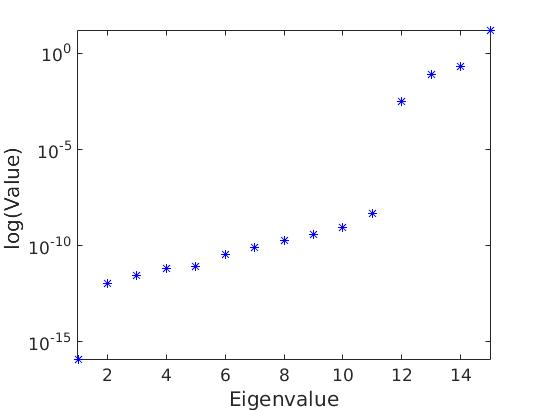
\includegraphics[width=5.5cm,height=5.5cm,keepaspectratio]
{images/eig_pod64.jpg}
%\vspace{-10pt}
\caption{Eigenvalues of the snapshot correlation matrix $\mathbf{R}=\mathbf{X}\mathbf{X}^T$, if 15 snapshots are used.}
\vspace{-5pt}
\label{fig:eig}
\end{wrapfigure}
We investigate the dependence on the contrast in permeability value between the layers for the ICCG and DICCG methods.
The permeability  $\sigma_2$ varies from $\sigma_2=10^{-1}mD$ to $\sigma_2=10^{-3}mD$. \\
Four wells are positioned in the corners with a bhp (bottom hole pressure) of -1 bar. One well is positioned in the center of the domain and has a bhp of +4 bars
(see Figure \ref{fig:hep_2}). Snapshots are obtained solving the system with different well
configurations (see Table \ref{table:sc}).

Table \ref{table:he22} shows the number of iterations required to reach convergence for the ICCG method and the deflation method with four linearly independent snapshots as deflation vectors DICCG$_{4}$, 15 linearly dependent snapshots DICCG$_{15}$ and the POD basis vectors, DICC$G_{POD_4}$\footnote{The * means that the solution is not reached within the maximum number of iterations allowed for the problem.}.
For the deflation vectors of DICCG$_{POD_4}$ we plot the eigenvalues of the snapshot correlation matrix $\mathbf{R}=\frac{1}{10}\mathbf{X}^T \mathbf{X}$ (see Section \ref{POD}) in Figure \ref{fig:eig}. We observe that there are 4 eigenvalues much larger than the rest. These largest eigenvalues are responsible for the slow convergence of the ICCG method. For the  DICCG$_{POD_4}$ method, we use the eigenvectors corresponding to the larger eigenvalues as deflation vectors.\\
\renewcommand{\arraystretch}{1}
\begin{table}[!ht]\centering
\begin{minipage}{.7\textwidth}
\vspace{10pt}
\centering
\begin{tabular}{ |c|c|c|c|} 
\hline
 $\sigma_2$ (mD) & $10^{-1}$& $10^{-2}$ & $10^{-3}$ \\
 \hline
  ICCG  & 90& 115&131\\ 
 
  DICCG$_4$  & 1 & 1& 1\\ 
  DICCG$_{15}$  & 200* & 200*& 200*\\
  DICCG$_{POD_4}$  & 1 & 1& 1\\
 \hline
\end{tabular}
\caption{Number of iterations for different contrast in the permeability of the layers
for the ICCG and DICCG methods.}
\label{table:he22}\end{minipage}
%\vspace{-10pt}
\end{table}

In Table \ref{table:he22}, for the ICCG method, we observe that the number of iterations 
increases if the contrast in the permeability increases. For the DICCG method with 4 linearly independent deflation vectors and 4 POD basis vectors, convergence is reached 
within one iteration and it does not change when we vary the contrast between permeability layers. However, for the case of 15 linearly dependent vectors, the solution is not reached within the 200 iterations, the maximum number of iterations allowed for this problem.\\

\emph{\textbf{SPE 10 model}}\\

\begin{wrapfigure}{R}{4.5cm}
\hspace{4mm}
 \centering
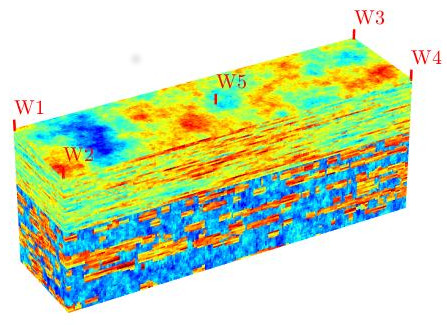
\includegraphics[width=4.5cm,height=4.5cm,keepaspectratio]
{images/perm85.jpg}
\caption{SPE 10 benchmark, permeability field.}
\label{fig:permcc}
\vspace{-10pt}

\end{wrapfigure}
This model has large variations in the permeability coefficients, the contrast between coefficients is $3\times 10^7$ \cite{Christie01}.
The model contains 60 x 220 x 85 cells (Figure \ref{fig:permcc}) and five wells, four of them located in the corners and one in the center of the domain.
Snapshots are obtained solving the system with different well
configurations (see Table \ref{table:sc}). As before, we simulate single-phase incompressible flow.\\
The number of iterations required to achieve convergence with the ICCG and DICCG methods for various grid sizes is presented in Table \ref{table:itgrid}. In this table, we observe that for the ICCG method we require 1011 iterations to reach the desired accuracy. Meanwhile, for the deflated methods DICCG$_4$ and DICCG$_{POD_4}$ only two iterations are required. In theory, only one iteration is necessary to reach the solution with the deflated methods. However, the large contrast in the permeability field may require higher accuracy for the snapshots to find the solution with deflation within one iteration within the imposed tolerance \cite{Diaz16}. In this case, the first iteration has a relative residual smaller than $10^{-10}$ for the DICCG$_4$ and DICCG$_{POD_4}$ methods, therefore after a first iteration we have already a good approximation.
\begin{table}[h!]
\centering
\begin{minipage}{.6\textwidth}
\centering
\begin{tabular}{|c | c| } 
 \hline
Method  &Iterations\\
   \hline
  ICCG &1011 \\ 
   DICCG$_{15}$ &  2000*\\ 
   DICCG$_{4}$ &  2\\  
   DICCG$_{POD_4}$  &2\\ 
\hline
\end{tabular}
\caption{Table with the number of iterations for ICCG and DICCG methods.}\label{table:itgrid}\end{minipage} 
\end{table}

For the deflated method with 15 linearly dependent snapshots (DICCG$_{15}$), we observe that the desired accuracy is not reached after 2000 iterations, as the deflation methods are linearly dependent, the deflation method is unstable because the matrix $E$ is a nearly singular matrix (reference to be added, new report).
\subsection{Compressible Problem}

\begin{wrapfigure}{R}{4.5cm}
\centering 
\vspace{-20pt}
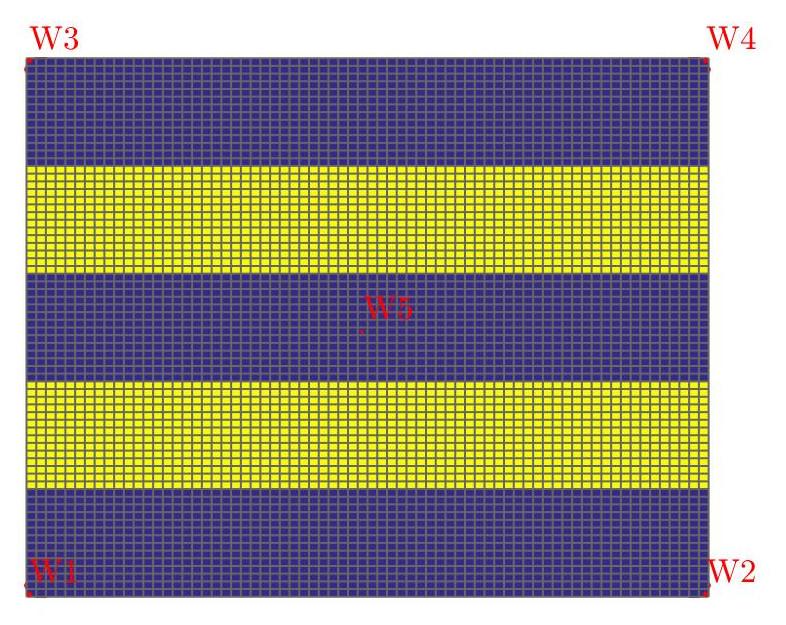
\includegraphics[width=4cm,height=4cm,keepaspectratio]{images/perm70.jpg}
 \vspace{-15pt}
\caption{ Heterogeneous permeability, 5 wells, compressible problem.}\label{fig:pc}
\vspace{-10pt}
\end{wrapfigure} 
In this section we model single-phase flow through a porous medium for a case when the density depends on the pressure 
according to Equation \eqref{eq:rhoeq}. We solve Equation \eqref{eq:ce5} for a fluid with the a compressibility of $c= 1 \times 10^{-3}$.
Equation \eqref{eq:ce5} is non-linear due to the dependence of the density on the pressure. Therefore, we need to 
linearize this equation via the Newton-Raphson (NR) method and to solve the resulting linear system. After linearization, we obtain the linear system \eqref{eq:lsJ} and we solve it with an iterative method; a summary of the procedure is presented in Algorithm 1. The simulation, with exception of the linear solvers, is performed with MRST. Automatic Differentiation (AD) is used for the NR loop \cite{Lie13}. The resulting linear system is solved with ICCG and DICCG methods. We compute the solution of the system for the first 10 time steps with the ICCG method. The rest of the time steps is solved with DICCG, using as deflation vectors the solution of the previous ten time steps and POD basis vectors computed from these solutions. The number of POD deflation vectors is specified for each problem. \\
We study an academic layered problem that consists of layers with two different permeability values 
(see Figure \ref{fig:pc}). The first layer has a permeability of $\sigma_1 = 30mD$, and the permeability 
of the second layer is varied; the permeability values of this second layer are $\sigma_2 =$ [3mD, 0.3mD, 0.03mD]. Therefore, the contrast between the layers 
is $10^{1},$ $10^{2}$ and $10^{3}$.
The domain is a square with five wells, four of which are positioned in the corners of the domain and one 
well in the center. The length of the domain is 70 m and the grid size is 35 grid cells in each dimension.  We impose homogeneous Neumann boundary conditions on all boundaries. \\
The initial pressure of the reservoir is set to 200 bars. The bottom hole pressure (bhp) in the corner wells is 100 bars and 
in the central well is 600 bars.  
The simulation was performed during 152 days with 52 time steps and a time step of 3 days. The tolerance of 
the NR method and the linear solvers is $10^{-5}$.\\
In Figure \ref{fig:compsol_1}, the solution obtained with the ICCG method is presented for a contrast in permeability layers of $10^{1}$. The upper left figure represents the pressure field at the final time step. The upper right 
figure represents the pressure across the diagonal joining the (1,1) and (35,35) grid cells for all the time steps. 
We observe the initial pressure (200 bars) across this diagonal and the evolution of the pressure field through time. 
In the lower figure, we observe the surface volume rate for the five wells during the simulation.

\begin{figure}[!h]
\centering
\hspace{-5mm}
\begin{minipage}{.5\textwidth}
 \centering
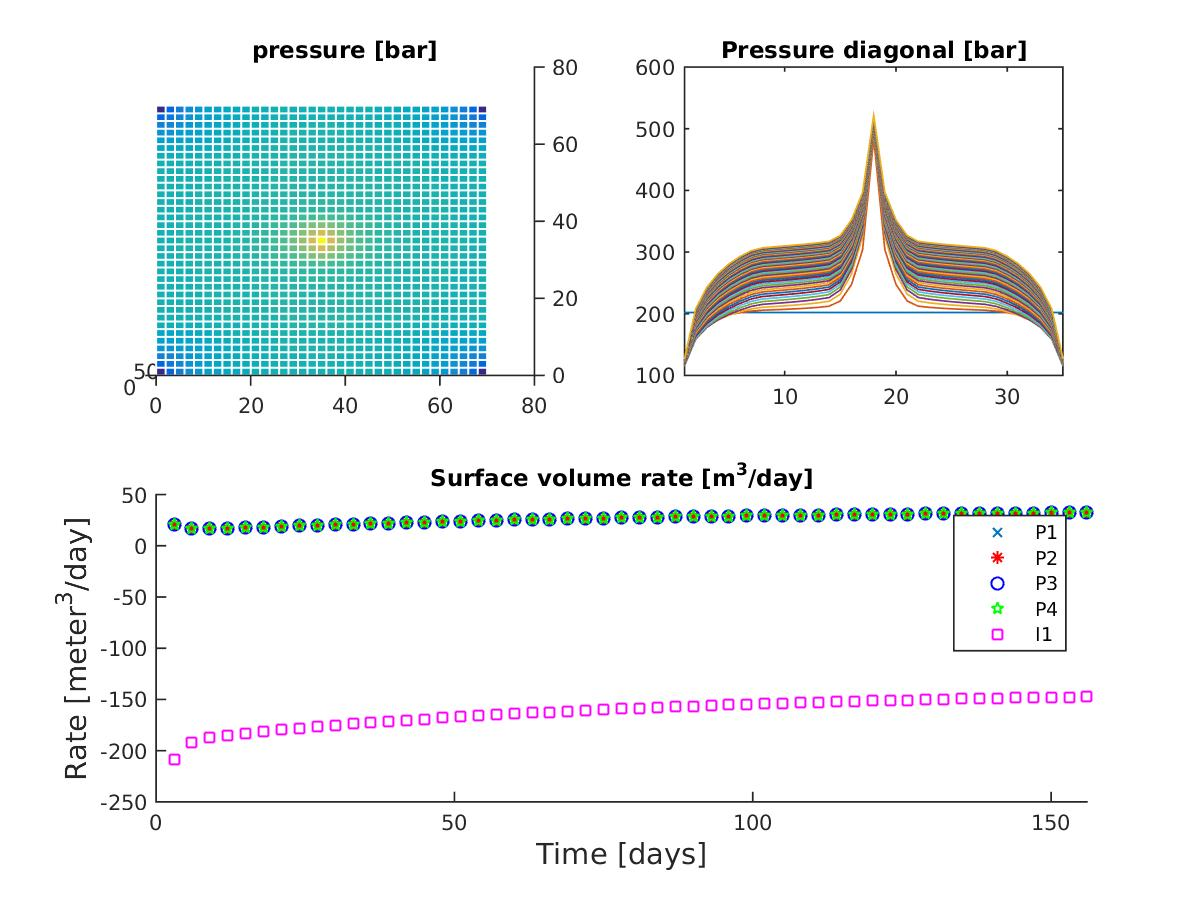
\includegraphics[width=7cm,height=7cm,keepaspectratio]
{images/solution.jpg}
\caption{Solution of the compressible problem solved with the ICCG method for a layered problem with a contrast between permeability layers of $10^{1}$.}
\label{fig:compsol_1}
\end{minipage}%
\hspace{5mm}
\begin{minipage}{.4\textwidth}
 \centering
 \vspace{5mm}
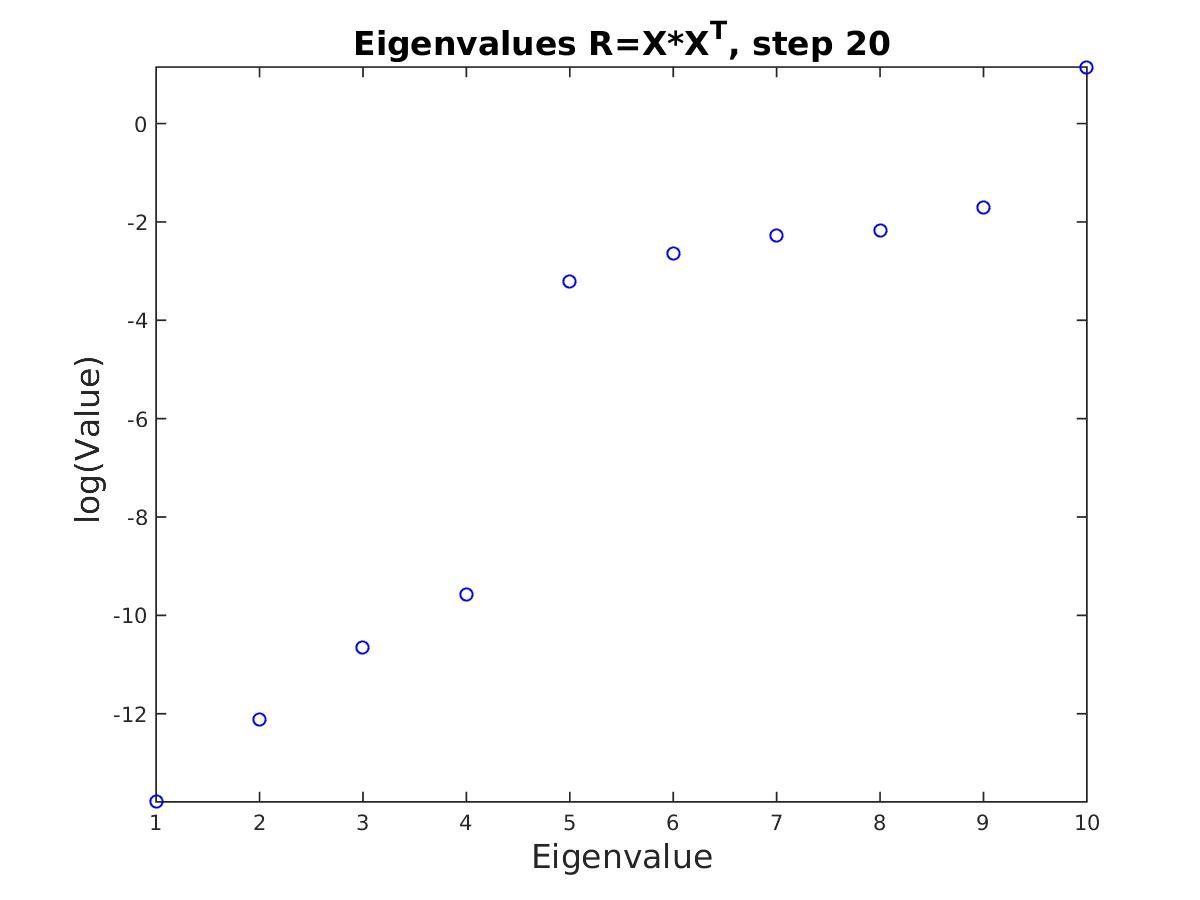
\includegraphics[width=5cm,height=5cm,keepaspectratio]{images/eig_pod2070.jpg}
\vspace{1mm}
\caption{Eigenvalues of the data snapshot correlation matrix $\mathbf{R}=\frac{1}{10}\mathbf{X}\mathbf{X}^T$, contrast between permeability layers of $10^{1}$.}
\label{fig:eig_POD_1}
\end{minipage}
\end{figure}
As mentioned before, for each time step, the previous 10 solutions are used as snapshots to compute the POD basis. The eigenvalues of the snapshot correlation matrix $\mathbf{R}=\frac{1}{10}\mathbf{X}\mathbf{X}^T$ constructed with the previous ten time steps are presented in Figure \ref{fig:eig_POD_1} for the 20$^{th}$ time step, for a contrast between permeability layers of $10$. In Figure \ref{fig:eig_POD_1}, we observe that six eigenvalues are larger than the rest. Then, we use the eigenvectors corresponding to these six eigenvalues as deflation vectors (DICCG$_{POD_6}$) to solve this problem. For a contrast between permeability layers of $10^{2}$ and $10^{3}$ we have 7 larger eigenvalues, therefore, we use 7 POD basis vectors as deflation vectors (DICCG$_{POD_7}$).  
For all the experiments, only the first time step requires more than two NR iterations. Hence, we solely study the behavior of the linear solvers during the first two NR iterations. \\
In Table \ref{table:litertot1} and Table \ref{table:litertot2} we compare the number of iterations necessary to reach convergence with the ICCG method and the deflation methods DICCG$_{10}$, DICCG$_{POD_6}$ and DICCG$_{POD_7}$.\\

\begin{table}[!ht]\centering
\begin{minipage}{1\textwidth}
\vspace{-10pt}
\centering
\begin{tabular}{ ||c|c||c|c|c|c|c||} 

\hline
\multicolumn{7}{|c|}{$1^{st}$ NR Iteration}  \\
\hline\
$\frac{\sigma_2}{\sigma_1}$&Total& Method & ICCG&DICCG &Total&\% of total\\
                           &   ICCG   &  & Snapshots& &ICCG& ICCG\\
 &     &  & & &+DICCG& \\
\hline
$10^{1}$ &780&DICCG$_{10}$ & 140&42& 182&23\\
 &780& DICCG$_{POD_6}$&140&84&  224&29\\
 \hline
$10^{2}$  &624&DICCG$_{10}$ &100&42&  142&23\\
          &624&DICCG$_{POD_7}$&100&42& 142 &23\\
          \hline
 $10^{3}$ &364&DICCG$_{10}$ &20&42  &62& 17\\
          &364&DICCG$_{POD_7}$&20&42&  62&17 \\
 \hline
 \end{tabular}
\caption{Comparison between the ICCC and DICCG methods of the average number of linear iterations for the first NR iteration for various contrast between permeability layers. }\label{table:litertot1}
\end{minipage}
\end{table}
For the first NR iteration (see Table \ref{table:litertot1}), we observe a significant reduction in the total number of linear iterations. 
For the case when we have a contrast between permeability layers of $10^{1}$ we observe that for the ICCG method, we need 780 linear iterations to compute the solution for the 52 time steps. By contrast, when we use the deflated method, we need 140 
linear iterations to compute the snapshots during the first ten time steps (computed with ICCG) and 42 and 84 for the 42 remaining time 
steps computed with DICCG$_{10}$ and DICCG$_{POD_6}$. Then, we need in total 182 and 224 linear iterations to compute the 
solution for the 52 time steps, which is 23\% and 29\% of the linear iterations required with only the ICCG method.\\
When we have a contrast in permeability of $10^{2}$, the required average of linear iterations to solve the 52 
time steps is 624 for the ICCG method. With the deflated methods, taking into account the computation of the snapshots, we require 
142 iterations for the DICCG$_{10}$ and  DICCG$_{POD_7}$ methods, which is the 23\% of the number of ICCG iterations. 
Finally, for a contrast between permeability layers of $10^{3}$ we require 364 linear iterations for the 52 time steps 
with the ICCG method. Meanwhile, the required iterations for the DICCG$_{10}$ and DICCG$_{POD_7}$ methods is 62. 
That is 17\% of the ICCG iterations (see Table \ref{table:litertot1}).\\

\begin{table}[!h]
\begin{minipage}{1\textwidth}
\vspace{-10pt}
\centering
\begin{tabular}{ ||c|c||c|c|c|c|c||} 

\hline
\multicolumn{7}{|c|}{$2^{nd}$ NR Iteration}  \\
\hline
$\frac{\sigma_2}{\sigma_1}$&Total&Method  & ICCG&DICCG &Total&\% of total\\
                           & ICCG     &  & Snapshots& &ICCG& ICCG\\
                           &     &  & & &+DICCG& \\
\hline
$10^{1}$ &988& DICCG$_{10}$&180&78&  258& 26\\
&988&DICCG$_{POD_6}$ &180&198&  378& 38\\
\hline
$10^{2}$&832&DICCG$_{10}$ &140&90&  230&28\\
&832&DICCG$_{POD_7}$&140&154&  294&33\\
\hline
$10^{3}$&884&DICCG$_{10}$&110&90&  200&23 \\
&884&DICCG$_{POD_7}$ &110&150&  260& 29\\
 \hline
 \end{tabular}
\caption{Comparison between the ICCC and DICCG methods of the average number of linear iterations for the second NR iteration for various contrast between permeability layers. }\label{table:litertot2}
\end{minipage}
\end{table}
For the second NR iteration (see Table \ref{table:litertot2}), we also observe a significant reduction in the total number of linear iterations.
For the case when we have a contrast between permeability layers of $10^{1}$, with the DICCG$_{10}$ and DICCG$_{POD_6}$ methods, it is necessary to perform only 26\% and 38\% of the linear iterations required with ICCG.\\
When we have a contrast in permeability layers of $10^{2}$, the required linear iterations are 28\% and 33\% of the ICCG iterations if we use the DICCG$_{10}$ and DICCG$_{POD_7}$ methods.
For a contrast between permeability layers of $10^{3}$, the DICCG$_{10}$ and DICCG$_{POD_7}$ methods require 23\%
and 29\% of the number of ICCG iterations. \\


\newpage
\textbf{SPE 10 model}\\
\begin{wrapfigure}{R}{5cm}
\centering 
\vspace{-10pt}
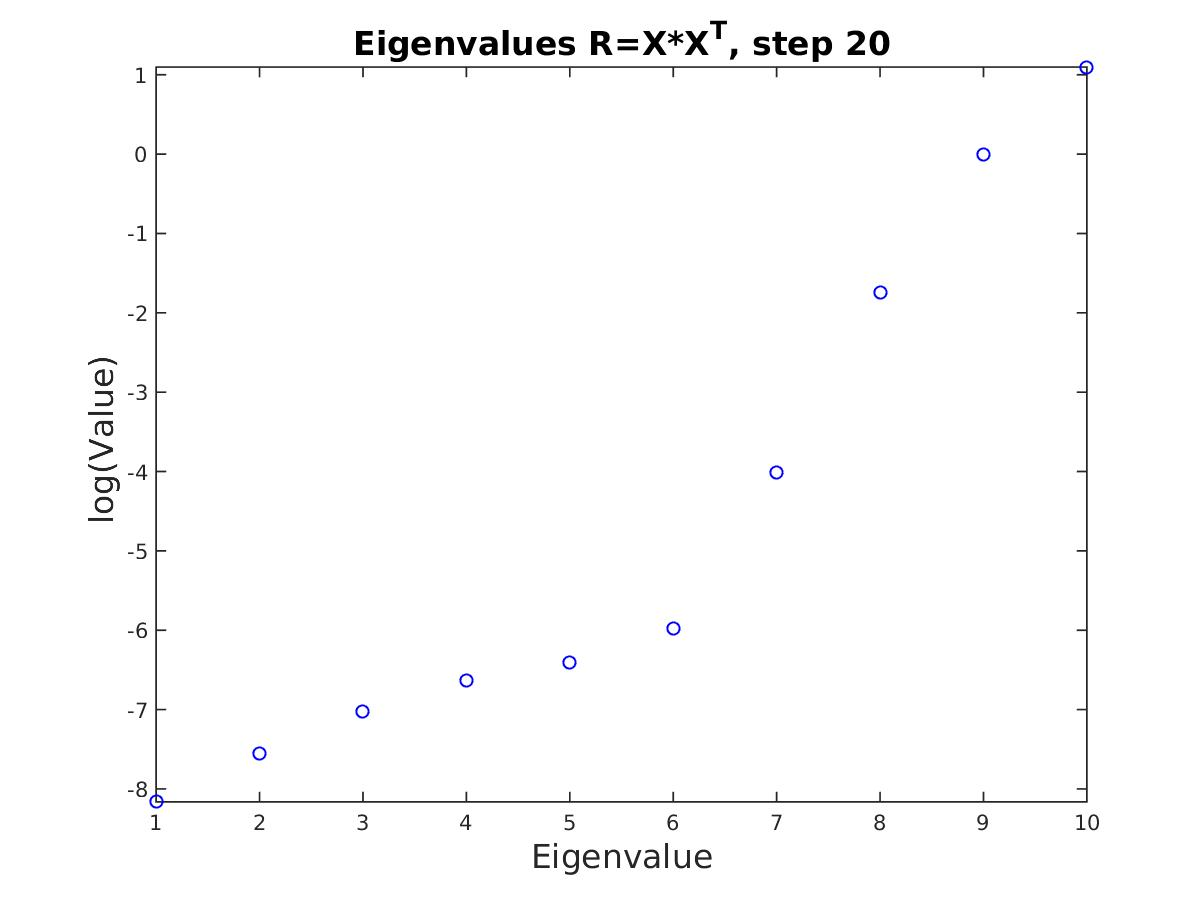
\includegraphics[width=5cm,height=5cm,keepaspectratio]{images/eig_pod2085.jpg}
%\vspace{-5mm}
\caption{Eigenvalues of the data snapshot correlation matrix $\mathbf{R}=\frac{1}{10}\mathbf{X}\mathbf{X}^T$, time step 20, full SPE 10 benchmark.}
\label{fig:eig_POD_SPE85}
\vspace{-5pt}
\end{wrapfigure}

We study the complete SPE 10 benchmark that consists of $60\times220\times85$ grid cells and has a contrast in permeability of $3\times 10^{7}$. To solve the linear system obtained after the NR linearization, we use 10 snapshots (the previous 10 time step solutions), and POD basis vectors as deflation vectors. The simulation was performed during 152 days with 52 time steps and a time step of 3 days.\\
In Figure \ref{fig:eig_POD_SPE85} the eigenvalues of the snapshot correlation matrix are presented. We observe that there are 4 eigenvalues larger than the rest, which implies that most of the information is contained in these eigenvalues. Therefore, we study the deflation method with 10 snapshots as deflation vectors and 4 POD basis vectors, the largest eigenvectors corresponding to the largest eigenvalues in Figure \ref{fig:eig_POD_SPE85}. \\


\begin{table}[!ht]\centering
\begin{minipage}{1\textwidth}
\vspace{-10pt}
\centering
\begin{tabular}{ ||c||c|c|c|c|c||} 
  \hline
   \multicolumn{6}{|c|}{$1^{st}$ NR Iteration}  \\
\hline
Total& Method &ICCG &DICCG &Total&\% of total\\
ICCG   &  & Snapshots& &ICCG& ICCG\\
       &  &          & & +DICCG& \\
\hline

10173&DICCG$_{10}$&1770&1134&2904&28 \\
10173 &DICCG$_{POD_4}$&1770&1554&3324&32  \\
\hline
 \end{tabular}
\caption{Average number of linear iterations for the first NR iteration, full SPE 10 benchmark.}\label{table:literspe1}
\end{minipage}
\end{table}
\begin{table}[!ht]\centering
\begin{minipage}{1\textwidth}
\vspace{-10pt}
\centering
\begin{tabular}{ ||c||c|c|c|c|c||} 
  \hline
   \multicolumn{6}{|c|}{$2^{nd}$ NR Iteration}  \\
\hline
Total& Method & ICCG&DICCG &Total&\% of total\\
ICCG   &  & Snapshots& &ICCG& ICCG\\
&  &          & & +DICCG& \\
\hline
10231&DICCG$_{10}$&1830&200&2030&20 \\
10231 &DICCG$_{POD_4}$&1830&200&2030&20 \\

\hline
 \end{tabular}
\caption{Average number of linear iterations for the second NR iteration, full SPE 10 benchmark.}\label{table:literspe2}
\end{minipage}
\end{table}
For the first NR iteration, we observe that the average number of iterations required for the ICCG method  is considerably reduced. For the ICCG method we require 10173 iterations for the first NR iteration and 10231 for the second (see Table \ref{table:literspe1} and Table \ref{table:literspe2}). With the deflated methods DICCG$_{10}$ and DICCG$_{POD_4}$, for the first NR iteration, we only need to perform 28\% and 32\% of the linear iterations required with the ICCG method.\\
For the second NR iteration, the deflated methods require only 20\% of the ICCG linear iterations. 
We also observe that for the first NR iteration we need 1770 linear iterations to compute the ten initial snapshots (computed with ICCG) and 1134 to compute the solution of the rest of the solutions (computed with DICCG). For the second NR iteration, the number of linear iterations is 1830 for the ten initial snapshots and 200 for the deflated methods. This shows that the largest amount of work is carried out for the computation of the snapshots obtained with the ICCG method, which is more evident for the second NR iteration.


\section*{Conclusions}
% Solving Partial Differential Equations for some applications can lead to the solution of large linear systems of equations that usually are the most time-consuming part of the solution. Iterative methods are known to be the best option to solve this large problem. However, sometimes the iterative methods are not sufficient to solve the problems in a reasonable amount of time and preconditioners become necessary to accelerate the convergence of these methods. As the systems become larger or ill-conditioned, new preconditioning techniques need to be developed to improve the performance of an iterative method. Some techniques like POD and deflation are combined with preconditioning to achieve a further acceleration.

In this work, we combine ICCG preconditioning with deflation and POD methods to accelerate the 
convergence of CG method for large systems and systems with high-contrast in permeability. 
The deflated Conjugated Gradient preconditioned with Incomplete Cholesky method (DICCG) is studied 
with $snapshots$, solutions of the system with diverse characteristics, and POD basis vectors as 
deflation vectors. \\
Flow through a porous medium is studied for an incompressible and a compressible fluid. We study an 
academic layer problem with different permeability values in the layers and the complete SPE 10 
benchmark problem (1,122,000 cells).\\
To solve the incompressible problem, we propose the use of solutions of the problem with different 
well configurations as deflation vectors. We observe that the number of linear iterations required with ICCG is reduced to only a few iterations with DICCG and this number is independent of the contrast in permeability for the deflation methods. Results also show that, if we have a linearly dependent set of deflation vectors, we have an unstable method that leads to a bad approximation of the solution. Combination of POD with deflation techniques is shown to be a way to obtain the main information about the system to speed-up the iterative method and to avoid instabilities.\\
For the compressible case, we propose the use of solutions of previous time steps, $snapshots$, 
and POD basis vectors computed from these snapshots as deflation vectors. 
With DICCG we reduce the number of iterations to around 25\% of 
the number of iterations of the ICCG method. We observe that the performance of the 
DICCG method with snapshots and POD basis vectors as deflation vectors is similar. The required 
number of POD basis vectors to achieve a good acceleration of the method depends on the problem. 
However, only a limited number of POD vectors is necessary to obtain a good speed-up 
(seven at most for the problems here studied). For the SPE 10 problem, we reduce the number of 
deflation vectors to 4 POD basis vectors, which can represent an important reduction in the number 
of operations required for the method. 
The deflation techniques here presented are not restricted to these methods and could be 
combined with different preconditioners, e.g. SSOR or AMG, and diverse iterative methods.



%\section{Bibliography styles}


\section*{References}

\bibliography{research}
\appendix
\section{List of notation}\label{a1}

\begin{table}[!h]
\centering
\begin{tabular}{c l l }
\hline
Symbol & Quantity & Unit \\[0.5ex]
\hline
$\phi$ & Rock porosity&   \\
 $\mathbf{K}$& Rock permeability&  $Darcy$ $(D)$ \\
 $c_r$& Rock compressibility&  $Pa^{-1}$ \\
$\mathbf{v}$ & Darcy's velocity& $ m/d$ \\
 $\alpha$& Geometric factor&   \\
$\rho$ &Fluid density &  $kg/m^3$ \\
 $\mu$&Fluid viscosity & $Pa \cdot s$   \\
${p}$  &Pressure &  $Pa$ \\
$g$  &Gravity &  $m/s^2$ \\
$d$ & Reservoir depth&  $m$ \\
$c_l$ &Liquid compressibility &  $Pa^{-1}$ \\
$q$ &Sources &   \\
\hline
\end{tabular}\label{table:symbols}
\caption{Notation}
\end{table}

\section{Stopping criteria}\label{a2}
When we use an iterative method, we always want that our approximation is close enough 
to the exact solution. In other words, we want that the error \cite[pag. 42]{Saad03}: 
$$||\mathbf{e}^k||_2=||\mathbf{x}-\mathbf{x}^k||_2,$$ or the relative error: 
$$\frac{||\mathbf{x}-\mathbf{x}^k||_2}{||\mathbf{x}||_2},$$is small. \\
When we want to chose a stopping criteria, we could think that the relative error is a
good candidate, but is has the disadvantage that we need to know the exact solution to compute it.
What we have instead is the residual $$\mathbf{r}^k=\mathbf{b}-\mathbf{A}\mathbf{x}^k,$$ 
that is actually computed in each iteration of the CG method. There is a relationship between the 
error and the residual that can help us with the choice of the stopping criteria.
$$\frac{||\mathbf{x}-\mathbf{x}^k||_2}{||\mathbf{x}||_2}\leq \kappa_2(A)\frac{||\mathbf{r}^k||_2}{||\mathbf{b}||_2}.$$
With this relationship in mind, we can choose the stopping criteria as an $\epsilon$ for which
$$ \frac{||\mathbf{r}^k||_2}{||\mathbf{b}||_2}\leq \epsilon.$$
But we should keep to have in mind the condition number of the matrix $\mathbf{A}$, because the relative error will be bounded by:
$$\frac{||\mathbf{x}-\mathbf{x}^k||_2}{||\mathbf{x}||_2}\leq \kappa_2(A) \epsilon.$$
\section{Singular Value Decomposition for POD}\label{a3}
If we perform SVD in $\mathbf{X}$, we obtain the following matrices \\
$\mathbf{X}=\mathbf{U}\Sigma \mathbf{V}^T, \qquad \mathbf{U}\in\mathbb{R}^{n \times n},\qquad \mathbf{\Sigma}\in\mathbb{R}^{n \times m}, \qquad \mathbf{V}\in\mathbb{R}^{m \times m}.$\\
To obtain the eigenvectors of $\mathbf{X}$, it is necessary to construct the matrix $\mathbf{R}= \mathbf{X}\mathbf{X}^T\in\mathbb{R}^{n \times n}$.\\ However, if the problem is large, the resulting matrix is large and the SVD can be expensive. Instead, we can compute the eigenvalues and eigenvectors from the much smaller matrix $\mathbf{R}^T= \mathbf{X}^T\mathbf{X}\in\mathbb{R}^{m \times m}$. For this matrix, the SVD is:
\begin{itemize}
\begin{minipage}{.4\textwidth}
\item[] $\mathbf{R}^T= \mathbf{X}^T\mathbf{X}$
 \item[] $\quad=(\mathbf{U}\Sigma \mathbf{V}^T)^T\mathbf{U}\Sigma \mathbf{V}^T$
 \item[] $\quad=\mathbf{V}\Sigma ^T\mathbf{U}^T\mathbf{U}\Sigma \mathbf{V}^T,$ $\mathbf{U}^T\mathbf{U}=\mathbf{I}$ 
  \item[] $\quad=\mathbf{V}\Lambda^T \mathbf{V}^T$, 
  $\Lambda^T=\Sigma ^T\Sigma \in\mathbb{R}^{m \times m}.$
\end{minipage}
\end{itemize}
From where we obtain $\mathbf{V}$ and $\Lambda^T$. Then we can compute $\mathbf{U}$ as follows:
$$\mathbf{U}=\mathbf{X}\mathbf{V}(\Lambda^T)^{-\frac{T}{2}}=\mathbf{X}\mathbf{V}(\Lambda^T)^{\frac{1}{2}},$$
that are the left-singular values of $\mathbf{X}.$


\section{Deflation method}\label{a4}
In this appendix, we explain how to obtain the solution of the linear system \eqref{eq:linsys} with deflation.
Some properties of the matrices used for deflation that will help us to find the solution of system \eqref{eq:linsys} are \cite{Tang09}:
\begin{enumerate}\label{defprop}
 \item[a)] $\mathbf{P}^2=\mathbf{P}.$
 \item[b)] $\mathbf{A}\mathbf{P}^T=\mathbf{P}\mathbf{A}.$
 \item[c)] $(\mathbf{I}-\mathbf{P}^T)\mathbf{x}=\mathbf{Q}\mathbf{b}.$
 \item[d)]$\mathbf{P}\mathbf{A}\mathbf{Q}=\mathbf{0}^{n\times n}.$
  \item[e)]$\mathbf{P}\mathbf{A}\mathbf{Z}=\mathbf{0}^{n\times l}.$
\end{enumerate}
To obtain the solution of the linear system \eqref{eq:linsys}, we start with the splitting:
\begin{equation}\label{eq:splx}
    \mathbf{x}=\mathbf{x}-\mathbf{P}^T\mathbf{x}+\mathbf{P}^T\mathbf{x}=(\mathbf{I}-\mathbf{P}^T)\mathbf{x}+\mathbf{P}^T\mathbf{x}.
\end{equation}
Multiplying expression \eqref{eq:splx} by $\mathbf{A}$, using the properties of the deflation matrices, we have:
\begin{align*}
\mathbf{A}\mathbf{x}&=\mathbf{A}(\mathbf{I}-\mathbf{P}^T)\mathbf{x}+\mathbf{A}\mathbf{P}^T\mathbf{x},\qquad&Property:\\
\mathbf{A}\mathbf{x}&=\mathbf{A}\mathbf{Q}\mathbf{b}+\mathbf{A}\mathbf{P}^T\mathbf{x},&c)\\
\mathbf{b}&=\mathbf{A}\mathbf{Q}\mathbf{b}+\mathbf{P}\mathbf{A}\mathbf{x},&b),
\end{align*}
multiplying by $\mathbf{P}$ and using the properties $\mathbf{P}\mathbf{A}\mathbf{Q}=
\mathbf{0}^{n\times n}$ and $\mathbf{P}^2=\mathbf{P}$, properties $d$) and $a$), we have:
\begin{align*}
\mathbf{P}\mathbf{A}\mathbf{Q}\mathbf{b}+\mathbf{P}^2\mathbf{A}\mathbf{x}&=\mathbf{P}\mathbf{b},\nonumber \\
\mathbf{P}\mathbf{A}\mathbf{x}&=\mathbf{P}\mathbf{b},
\end{align*}
where $\mathbf{P}\mathbf{A}\mathbf{x}=\mathbf{P}\mathbf{b}$ is the deflated system. Since 
$\mathbf{P}\mathbf{A}$ is singular, the solution of Equation \eqref{eq:defsys} can contain
components of the null space of $\mathbf{P}\mathbf{A}$, ($\mathcal{N}(\mathbf{P}\mathbf{A})$). A solution of this system, called the deflated
solution, is denoted by $\mathbf{\hat{x}}$. Then, the linear system to solve is:\\
\begin{align}\label{eq:defsys}
\mathbf{P}\mathbf{A}\hat{\mathbf{x}}&=\mathbf{P}\mathbf{b}.
\end{align}
As the solution of Equation \eqref{eq:defsys} can contain components of 
$\mathcal{N}(\mathbf{P}\mathbf{A})$,
$\mathbf{\hat{x}}$ can be decomposed as:
\begin{equation}\label{eq:xxy}
\mathbf{\hat{x}}=\mathbf{x}+ \mathbf{y},
\end{equation}
with $\mathbf{y} \in \mathcal{R}(\mathbf{Z})\subset \mathcal{N}(\mathbf{P}\mathbf{A}),$ 
and $\mathbf{x}$ the solution of Equation \eqref{eq:linsys}.\\
Note: If $\mathbf{y} \in \mathcal{R}(\mathbf{Z}),$ then $$\mathbf{y}=\sum^{m}_{i=1}\alpha_i \mathbf{z}_i,$$\\
 \begin{equation*}\label{eq:paz}
 \mathbf{P}\mathbf{A}\mathbf{y} =\mathbf{P}\mathbf{A}(\mathbf{z}_1\alpha_1 +...+ \mathbf{z}_m\alpha_m)=\mathbf{P}\mathbf{A}\mathbf{Z}\mathbf{\alpha},\end{equation*}
 from property e) we have:
 \begin{equation*}\label{eq:pay}
 \mathbf{P}\mathbf{A}\mathbf{y}=\mathbf{0}.
 \end{equation*}
Therefore $\mathcal{R}(\mathbf{Z})\subset \mathcal{N}(\mathbf{P}\mathbf{A}),$ and using property b) we have:
 \begin{equation*}
 \mathbf{P}\mathbf{A}\mathbf{y}=\mathbf{A}\mathbf{P}^T\mathbf{y}=\mathbf{0}.
 \end{equation*}
 As $\mathbf{A}$ is invertible, we have:
  \begin{equation}\label{eq:py}
\mathbf{P}^T\mathbf{y}=\mathbf{0}.
 \end{equation}
 Multiplying Equation \eqref{eq:xxy} by $\mathbf{P}^T$ we obtain:
$$\mathbf{P}^T\mathbf{\hat{x}}=\mathbf{P}^T\mathbf{x}+\mathbf{P}^T\mathbf{y}.$$
substituting Equation \eqref{eq:py} we arrive to:
  \begin{equation}\label{eq:ptx}
\mathbf{P}^T\mathbf{\hat{x}}=\mathbf{P}^T\mathbf{x}.
 \end{equation}
Substitution of Equation \eqref{eq:ptx} and property c) in Equation \eqref{eq:splx} leads to:
\begin{equation}\label{eq:xfromxh1}
    \mathbf{x}=\mathbf{Q}\mathbf{b}+\mathbf{P}^T\mathbf{\hat{x}}, 
\end{equation}
which gives us the relation between $\mathbf{\hat{x}}$ and $\mathbf{x}$.
\end{document}